% this document is based on Máté Cserép https://github.com/mcserep/elteikthesis work and Zoltán Istenes modifications, extensions (2023), specially created for the IFRoS students

\PassOptionsToPackage{loadshadowlibrary}{todonotes}
\documentclass[
	parspace, % Add vertical space between paragraphs
	noindent, % No indentation of first lines in each paragraph
	%nohyp, % No hyphenation of words
	%twoside, % Double sided format
	%draft, % Quicker draft compilation without rendering images
	final, % Set final to hide todos
]{elteikthesis}

% The minted package is also supported for source highlighting
% See minted-integration.tex for example
%\usepackage[newfloat]{minted}

\usepackage{graphicx}
\usepackage{amsmath, amssymb}
\usepackage{listings}
\usepackage{longtable}
\usepackage{multirow}
\usepackage{float}
\usepackage{caption}
\usepackage{subcaption}
\usepackage{enumitem}
\usepackage{hyperref}
\usepackage{afterpage}
\usepackage{titlesec}

% Document's metadata
\title{Active Visual Search for Object Localization for Boston Dynamic SPOT robot} % title
\date{2026} % year of defense

% Author's metadata
\author{Lorenz Killer}
\degree{Intelligent Field Robotics Systems - IFRoS MSc}

% Supervisor(s)' metadata
\supervisor{Dr. Zoltán ISTENES} % internal supervisor's name
\affiliation{Associate Professor, ELTE} % internal supervisor's affiliation

\extsupervisor{PhD. András MAJDIK} % external supervisor's name
\extaffiliation{Senior Researcher, HUNREN Sztaki} % external supervisor's affiliation

\secondextsupervisor{MSc. Sándor Gazdag}
\secondextaffiliation{Research Associate, HUNREN Sztaki}

% University's metadata
\university{Eötvös Loránd University} % university's name
\faculty{Faculty of Informatics} % faculty's name
\department{Erasmus Mundus Joint Master in \\Intelligent Field Robotic Systems} % department's name... -> programme name
\city{Budapest} % city
\logo{elte_cimer_szines} % logo

% Add bibliography file
\addbibresource{elteikthesis.bib}

% The document
\begin{document}

% Set document language
%\documentlang{hungarian}
\documentlang{english}

% List of todos (not in the final document)
% \listoftodos[\todolabel]

% Title page (mandatory)
\maketitle
% Topic declaration page (mandatory) - can also be attached instead
% \includepdf{topicdeclaration.pdf}

% --- ABSTRACT ---
\pagenumbering{roman}
\chapter*{Abstract}
\addcontentsline{toc}{chapter}{Abstract} % This line is optional, but recommended if you want it in the TOC

Autonomous mobile robots increasingly require the ability to explore unknown environments and locate target objects. These abilities are necessary for applications ranging from industrial inspection to search and rescue operations. Traditionally exploration strategies rely on fixed cameras firmly attached to the robot, coupling the Field of View with the robot's base heading.
This thesis introduces an active visual search pipeline designed for mobile robotic platforms equipped with Pan-Tilt-Zoom (PTZ) cameras. The proposed framework integrates real-time object detection with 3D occupancy mapping and tracks the estimated object locations using a factor graph. A custom, modular ROS~2 software architecture was developed. It was evaluated in a simulated warehouse as well as a real-world office environment deploying the Boston Dynamics Spot robot. 
Experimental results compare three exploration strategies: passive search, active search, and active search with landmark zoom confirmation. The results show that actively coordinating base mobility while independently controlling the PTZ gaze can enhance object localization accuracy and target detection confidence. Furthermore, by leveraging optical zoom for long-range target verification, the active pipeline can reduce unnecessary physical base movement, decreasing total battery consumption and potentially improving the total operation time of the robotic platform.
\cleardoublepage

% Table of contents (mandatory)
\tableofcontents
\cleardoublepage

% Acknowledgements (optional) - in case your thesis received funding or would like to express special thanks to someone
% \todo{Acknowledgemenets}
% \chapter*{\acklabel}
% \addcontentsline{toc}{chapter}{\acklabel}
% In case your thesis received financial support from a project or the university, it is usually required to indicate the proper attribution in the thesis itself\footnote{Erasmus Mundus Joint Master in Intelligent Field Robotic Systems...}. Special thanks can also be expressed towards teachers, fellow students and colleagues who helped you in the process of creating your thesis.
\bigskip

% Using the IMRaD structure  (\url{https://en.wikipedia.org/wiki/IMRAD}) is usually a very good starting point. Try to follow and adapt if needed.

\cleardoublepage
\clearpage 
\pagenumbering{arabic}

% Main content

\chapter{Introduction}
\label{ch:intro}

The ability to autonomously navigate unknown environments and locate specific targets is an important capability for autonomous mobile robots. From search and rescue operations in disaster zones to industrial inspection and warehouse logistics, robotic agents are increasingly tasked with finding objects in complex, unstructured spaces. Existing robotic exploration methods employ sensors rigidly attached to the robots, forcing the system to couple its perception entirely with its base heading. This comes with two limitations for search efficiency: first, the robot must change its base trajectory to scan its surroundings and second, relying on fixed-focal-length cameras restricts the resolution at long distances. This forces the robot to physically approach targets to confirm their identity.

\section{Motivation}
While current research has explored the concepts of object search thoroughly, these studies typically use single cameras fixedly mounted on a mobile base, sometimes in combination with a LiDAR sensor for depth inference. However, modern robotic platforms are capable of hosting highly sophisticated, mechanically independent sensor suites. 

The focus of this thesis is to use a Pan-Tilt-Zoom (PTZ) camera mounted on the Boston Dynamics Spot\footnote{\url{https://bostondynamics.com/products/spot/}} to guide in active search. PTZ cameras introduce a crucial degree of freedom in visual search, allowing the robot's "gaze" to be controlled independently of its "body." By using this hardware, we aim to demonstrate that the state-of-the-art in robotic object localization can be augmented through applied engineering. Integrating active gaze control with trajectory planning promises to yield a more efficient and versatile solution for real-world search operations.

\section{Problem Statement}
Active visual search requires an agent to decide both where to move and where to look. This needs coordination of base mobility and independent camera gaze. Mechanically steerable cameras introduce extra sensing degrees of freedom that affect coverage, resolution, and detection reliability. The core challenge is to design a pipeline that models measurement uncertainty across different viewpoints and zoom settings, projects detections into a 3D representation, robustly associates them with previously seen objects and uses these detection to estimate object locations. Base navigation and gaze should be controlled to maximize detection confidence while minimizing unnecessary motion during an exploration and object search task.

\section{Objectives}
The primary objective of this thesis is to formulate, implement, and evaluate an active visual search pipeline for dynamic PTZ-equipped robots. To achieve this, the project delivers two main contributions:
\begin{enumerate}
    \item \textbf{Algorithmic Proof of Concept:} A complete perception and optimization pipeline that leverages 2D object detections, projects them into 3D space using ray casting inside probabilistic occupancy maps, and robustly tracks the corresponding landmark states using a factor graph.
    \item \textbf{Extensible Software\footnote{\url{https://master-thesis.lolo.place}}:} The development of a modular, hardware-agnostic ROS~2 software package. The resulting framework provides ready-to-use PTZ control and exploration interfaces for the Boston Dynamics Spot robot, a complete Gazebo-based simulation environment, and extensible core nodes that can be deployed on any mobile base utilizing the Nav2 stack.
\end{enumerate}

\section{Research questions}

\begin{enumerate}
	\item How can a robotic agent autonomously coordinate base mobility and independent camera gaze to maximize the probability of detecting a target object in an unknown environment?

	\item How can the trade-off between sensor coverage (Field of View) and detection confidence (Resolution) be modeled?

	\item How can an active visual search strategy improve search efficiency and detection range compared to standard passive exploration baselines?
\end{enumerate}
        
\section{Scope and Limitations}
This research touches several topics currently investigated by the scientific community. This includes Simultaneous Localization and Mapping (SLAM), global exploration and next-best-view planning. To maintain focus on the implementation and algorithmic optimization of the active object search, some constraints are applied. 

For simplicity, experiments and planning assume a single-level (planar) environment: navigation and frontier selection operate on a 2D projected map while 3D obstacles are retained for visibility and collision reasoning. Environments are additionally assumed to be static, not having any obstacles or other agents moving inside of them except the robot itself.

The main goal of this thesis is to develop a working real-world system on the Boston Dynamics Spot robot. Therefore, robot state localization is treated as a given, leveraging the robot's built-in advanced visual odometry and pose estimates. Furthermore, object recognition assumes the usage of a pre-trained deep learning object detector, meaning the scope relies on the accuracy of the underlying detection model and its bounding-box detections.

\pagebreak
\section{Thesis structure}
The rest of this thesis is structured as follows:

\begin{description}
    \item[Chapter~\ref{ch:lit-review}: Literature Review] reviews the state-of-the-art literature concerning active SLAM, autonomous visual search, and the application of pan-tilt-zoom cameras in mobile robotics.
    \item[Chapter~\ref{ch:methodology}: Methodology] details the modular software architecture and algorithms used for the active visual search system, encompassing mapping, navigation, object detection, and state optimization.
    \item[Chapter~\ref{ch:experiments}: Experiments] outlines the physical and simulated testing environments, detailing the hardware setup of the Boston Dynamics Spot robot and the complementary simulation configuration in Gazebo.
    \item[Chapter~\ref{ch:results}: Results and Discussion] presents the experimental outcomes, evaluating the system's performance, search efficiency, and reliability against the defined evaluation metrics.
    \item[Chapter~\ref{ch:conclusion}: Conclusion] summarizes the core findings, revisits the initial research questions, highlights the project's contributions, and outlines potential avenues for future work.
\end{description}

Finally, the appendix provides supplementary material, including a declaration regarding the use of Artificial Intelligence tools (Appendix~\ref{app:ai-usage}), as well as in-depth plots of the experimental results (Appendix~\ref{app:in-depth-results}).

\chapter{Literature Review}
\label{ch:lit-review}

Placed et al.~\cite{survey_placed_2023} synthesize recent research on robotic exploration, active exploration, the next-best-view problem and more under the unifying framework of \textit{Active Simultaneous Localization and Mapping (SLAM)}. They formalize the task mathematically and decompose it into three core stages: generating candidate actions, computing their utility, and selecting and executing an action. They then review and categorize prior work according to the underlying methodological choices. A condensed and focused summary for this thesis as well as some more recent and relevant works are presented in Section \ref{sec:lit-review-slam}

In addition, relevant works on the broad topic of active search are reviewed in Section~\ref{sec:lit-review-search}. These studies show how search policies must reason about perception, motion, and uncertainty to efficiently locate target objects. 

Active search naturally motivates closer attention to sensing configurations that can actively direct gaze in addition to the robots base pose. Thus relevant literature specifically focused on Pan-Tilt-Zoom cameras is discussed in Section~\ref{sec:lit-review-ptz}. This includes early work on PTZ control, surveillance applications, visual object tracking and systems that integrate PTZ cameras with mobile robotic platforms.

\section{Exploration and active SLAM}
\label{sec:lit-review-slam}

Yamauchi \cite{frontierbased_yamauchi_1997} introduced the concept of frontiers for autonomous exploration. Conceptually, frontiers are regions on the boundary between known and unexplored areas. They show that identifying and pursuing such frontiers is a feasible and sufficient approach for exploring arbitrary unknown environments. Based on their work, several papers \cite{efficient_keidar_2014, approaches_quin_2021} focused on more efficient methods to detect such frontiers, while others \cite{multiresolution_batinovi_2021, frontierbased_deng_2020, autonomous_umari_2017, receding_bircher_2016} worked towards efficient methods to make frontier-based exploration feasible in 3D.

A limitation of the mentioned works so far is their expected sensor setup. Most works focus on the theoretical capabilities considering a single, most commonly RGBD, camera. Real robotic platforms rarely have this limitation and can mount a multitude of cameras and other sensors that can all be leveraged to their advantage. This gap has been addressed by works such as Kuo et al. \cite{redesigning_kuo_2020} and Kaveti et al. \cite{design_kaveti_2022}, which improve existing SLAM systems by a more general multi-camera model. In their very recent paper Malczyk et al. \cite{reinforcement_malczyk_2026} equip a flying robot platform with a pan and tilt camera and utilize it for navigation. Their approach is based on reinforcement learning and resembles more a local waypoint planner than a full fledged navigation or exploration system.

While all aforementioned works consistently improved on the active SLAM problem they all chose to see exploration as merely the act of uncovering as much geometric area (or volume in the case of 3D explorations) as possible. This makes the need obvious to extend the problem further to include semantic information in order to allow advanced reasoning within the scene representation. Asgharivaskasi et al. \cite{semantic_asgharivaskasi_2023} as well as Zhang et al. \cite{active_zhang_2024} tackle this endeavour by including semantic information provided by modern segmentation frameworks. This leads to rich map representations easily interpreted by humans and ready to be used for advanced reasoning for robotic agents. Both of these approaches trivially allow the problem of object search to be solved by searching in the resulting map, but neither of them guide exploration to more effectively find desired objects in a scene. For this reason, the theoretical background of this thesis also has to take into consideration literature about active search (see Section \ref{sec:lit-review-search}).

\section{Active search}
\label{sec:lit-review-search}

Bajcsy et al. \cite{revisiting_bajcsy_2018} broadly describe the topic of active sensing as "a problem of an intelligent data acquisition process" and more specifically the goal of active search as "the optimization task of selecting the set of robot actions that maximize the probability of finding a target within cost constraints". 

Several early works have tried to solve this problem using traditional methods. Fekete et al. \cite{online_fekete_2006} for example tackled online search using a mobile robot equipped with a 3D laser scanner, relying on a basic "stop, scan, plan, go" strategy without prior knowledge of the environment. Tsotsos and Shubina \cite{attention_tsotsos_2007} advanced this by introducing programmatic visual attention mechanisms—using low-level image features to determine mapping saliency—to reduce the search space and prioritize where the camera should look based on probabilities. Sjöö et al. \cite{object_sj_2009} built on view planning by using a navigation graph and an occupancy grid. They utilized traditional, handcrafted computer vision methods: using Scale-Invariant Feature Transform (SIFT) for matching keypoints to recognize objects, combined with heuristic visual saliency models (attention) to highlight relevant image regions and estimate distances. Shubina and Tsotsos \cite{visual_shubina_2010} then explicitly divided the search task into "where to look next" and "where to move next" within a 3D grid environment, constantly updating a target probability map using a stereo camera. Finally, Aydemir et al. \cite{active_aydemir_2013} advanced the field by considering spatial semantics - like reasoning that a coffee cup is usually in a kitchen - to more efficiently find target objects across large, previously unexplored areas.


While these foundational methods established the core principles of active search, many of their traditional visual techniques have been rendered obsolete by more recent advances in deep image processing. More modern approaches have shifted towards leveraging deep vision networks to tackle the object search problem and handle increasingly complex environments, probabilistic uncertainties, and limitations of real-world sensors. 
Dang et al. \cite{autonomous_dang_2018} integrated Convolutional Neural Networks into their planner for aerial robots, projecting detections onto a 3D occupancy map to actively maximize the observation resolution of target objects. To manage the computational complexity of such probabilistic environments, Wang et al. \cite{efficient_wang_2018} modeled the search as a Partially Observable Markov Decision Process. Their approach significantly reduced the state-space and improves path-planning efficiency Addressing the practical execution, Schmid et al. \cite{explore_schmid_2019} proposed a Deep Reinforcement Learning framework that breaks the process down into three distinct subtasks: exploration, approaching, and active termination. Rasouli et al. fused visual attention models to bias the robot's decisions toward relevant visual stimuli, preventing exhaustive scanning of the environment. Finally, addressing the unreliability of real-world vision pipelines, Taioli et al. \cite{unsupervised_taioli_2023} recently introduced an unsupervised method that specifically accounts for false positives and miss-detections. Their system achieves robust active visual search without the need for extensive offline training data.

A recent study by Wu et al. \cite{realworld_wu_2025} recorded how humans tackle object search in unknown environments and found that subjects rely not only on changing their body position but also to a high degree on eye as well as head movements. This suggests that similar methods might be useful for robotics agents. For this reason literature on Pan-Tilt-Zoom cameras is reviewed in the next Section.

\section{Pan-Tilt-Zoom Cameras}
\label{sec:lit-review-ptz}

Early literature \cite{tutorial_hutchinson_1996, visual_chaumette_2006, visual_chaumette_2007} mostly focused on robotic manipulator control systems, which were coupled with a camera on the manipulator itself. More recently Nebeluk et al. \cite{predictive_nebeluk_2023} picked up their work and developed a modern system to track objects and facilitate grasping. While some of these concepts are relevant for this thesis, the control of a mobile base mounted with a PTZ camera is fundamentally different and many visual methods from the past are obsolete due to the advances in deep image processing.

By far the biggest area of research regarding PTZ cameras is surveillance. A number of papers can be found focusing on anomaly detection \cite{anomalous_lpezrubio_2021}, coverage maximization of multi-camera systems \cite{voronoibased_arslan_2018} or overall detection and recognition accuracy maximization \cite{collaborative_krahnstoever_2008, autonomous_davani_2021}. They all assume the PTZ cameras as unable to move within the scene.

Others have focused their works more on tracking objects within a scene. You et al. \cite{cellbased_you_2022} used a PTZ camera in a known scene to track and infer 3D localization estimates of a tracked objects. Li et al. \cite{camera_li_2021} designed a system that aims to keep a predefined object within the center of a PTZ camera while maximizing the zoom without loosing track of the object. They mention that such a system could also be mounted on a mobile robot, yet do not verify this with experiments. Wang et al. \cite{target_wang_2019} use a monocular PTZ camera for target tracking using classical computer vision methods like color and edge recognition and infer the distance from the camera to the target using the PTZ cameras physical geometry with structure from motion. While they deploy their system on a mobile humanoid dual-arm robot, they don't cover base movement nor manipulation in their paper.

More closely related to this thesis are two approaches that both combine an omnidirectional camera with a PTZ camera on a moving platform. Yu et al. \cite{visual_yu_2010} detect and track moving objects from wide-angle images and then use the PTZ camera to zoom in for face detection while the base follows the target. Similarly, Fahn and Lo \cite{highdefinition_fahn_2010} use an omnidirectional camera to localize faces and then rapidly steer and zoom a PTZ camera for high-resolution capture. Both works show that pairing 360\textdegree coverage with PTZ zoom helps mitigate the resolution limits of omnidirectional tracking, yet they lack integration into more sophisticted navigation or exploration pipelines.

Regarding the selection of an adequate zoom levels Denzler et. al \cite{information_denzler_2003} propose a controller model  that dynamically selects the zoom level to minimize the object's 3D state uncertainty. Building on this for real-world applications, Tordoff et al. \cite{reactive_tordoff_2007} introduce a reactive controller that keeps the target within the camera's field of view while also compensating for hardware delays.

Finally another important factor about PTZ cameras is camera calibration. Due to the nature of mechanical movements and zooming a PTZ camera can accumulate a significant localization error over time. Wu et. al \cite{keeping_wu_2013} as well as Lisanti et. al \cite{continuous_lisanti_2016} propose two different methods of keeping a PTZ camera calibrated also under a long uptime.

\section{Research Gap}
This research review shows an overview over three different areas of research that are mostly studied in separation. This thesis aims to bring the worlds together and demonstrate a system that is capable of performing both exploration and active search with a PTZ camera. We present a possible software layout that manages to coordinate both base movement as well as PTZ camera control and demonstrate a baseline implementation that compares classical "passive" methods with an active PTZ-camera based one and shows which benefits come with that.

\chapter{Methodology}
\label{ch:methodology}

This chapter explains the different software modules, how they interact with each other, and why certain design decisions were made. We start by outlining an overview in Section~\ref{sec:software} and then examine in detail each component in the following sections.

\section{Software Design}
\label{sec:software}
A high-level overview of the system's data flow is shown in Figure~\ref{fig:software_diagram}. As inputs, the architecture accepts any number of RGB image streams from the robot's onboard cameras, alongside depth information in the form of a 3D point cloud. This way the system is agnostic to the robots concrete hardware; it functions whether the platform is equipped solely with the active PTZ camera or features additional static body cameras. Similarly, the required 3D spatial data can be sourced from RGB-D cameras, a dedicated LiDAR sensor, or a combination of both. The outputs of the modular, concurrent system are two command streams: one for controlling the robot's base movement and one for PTZ camera control.

\begin{figure}[H]
    \centering
    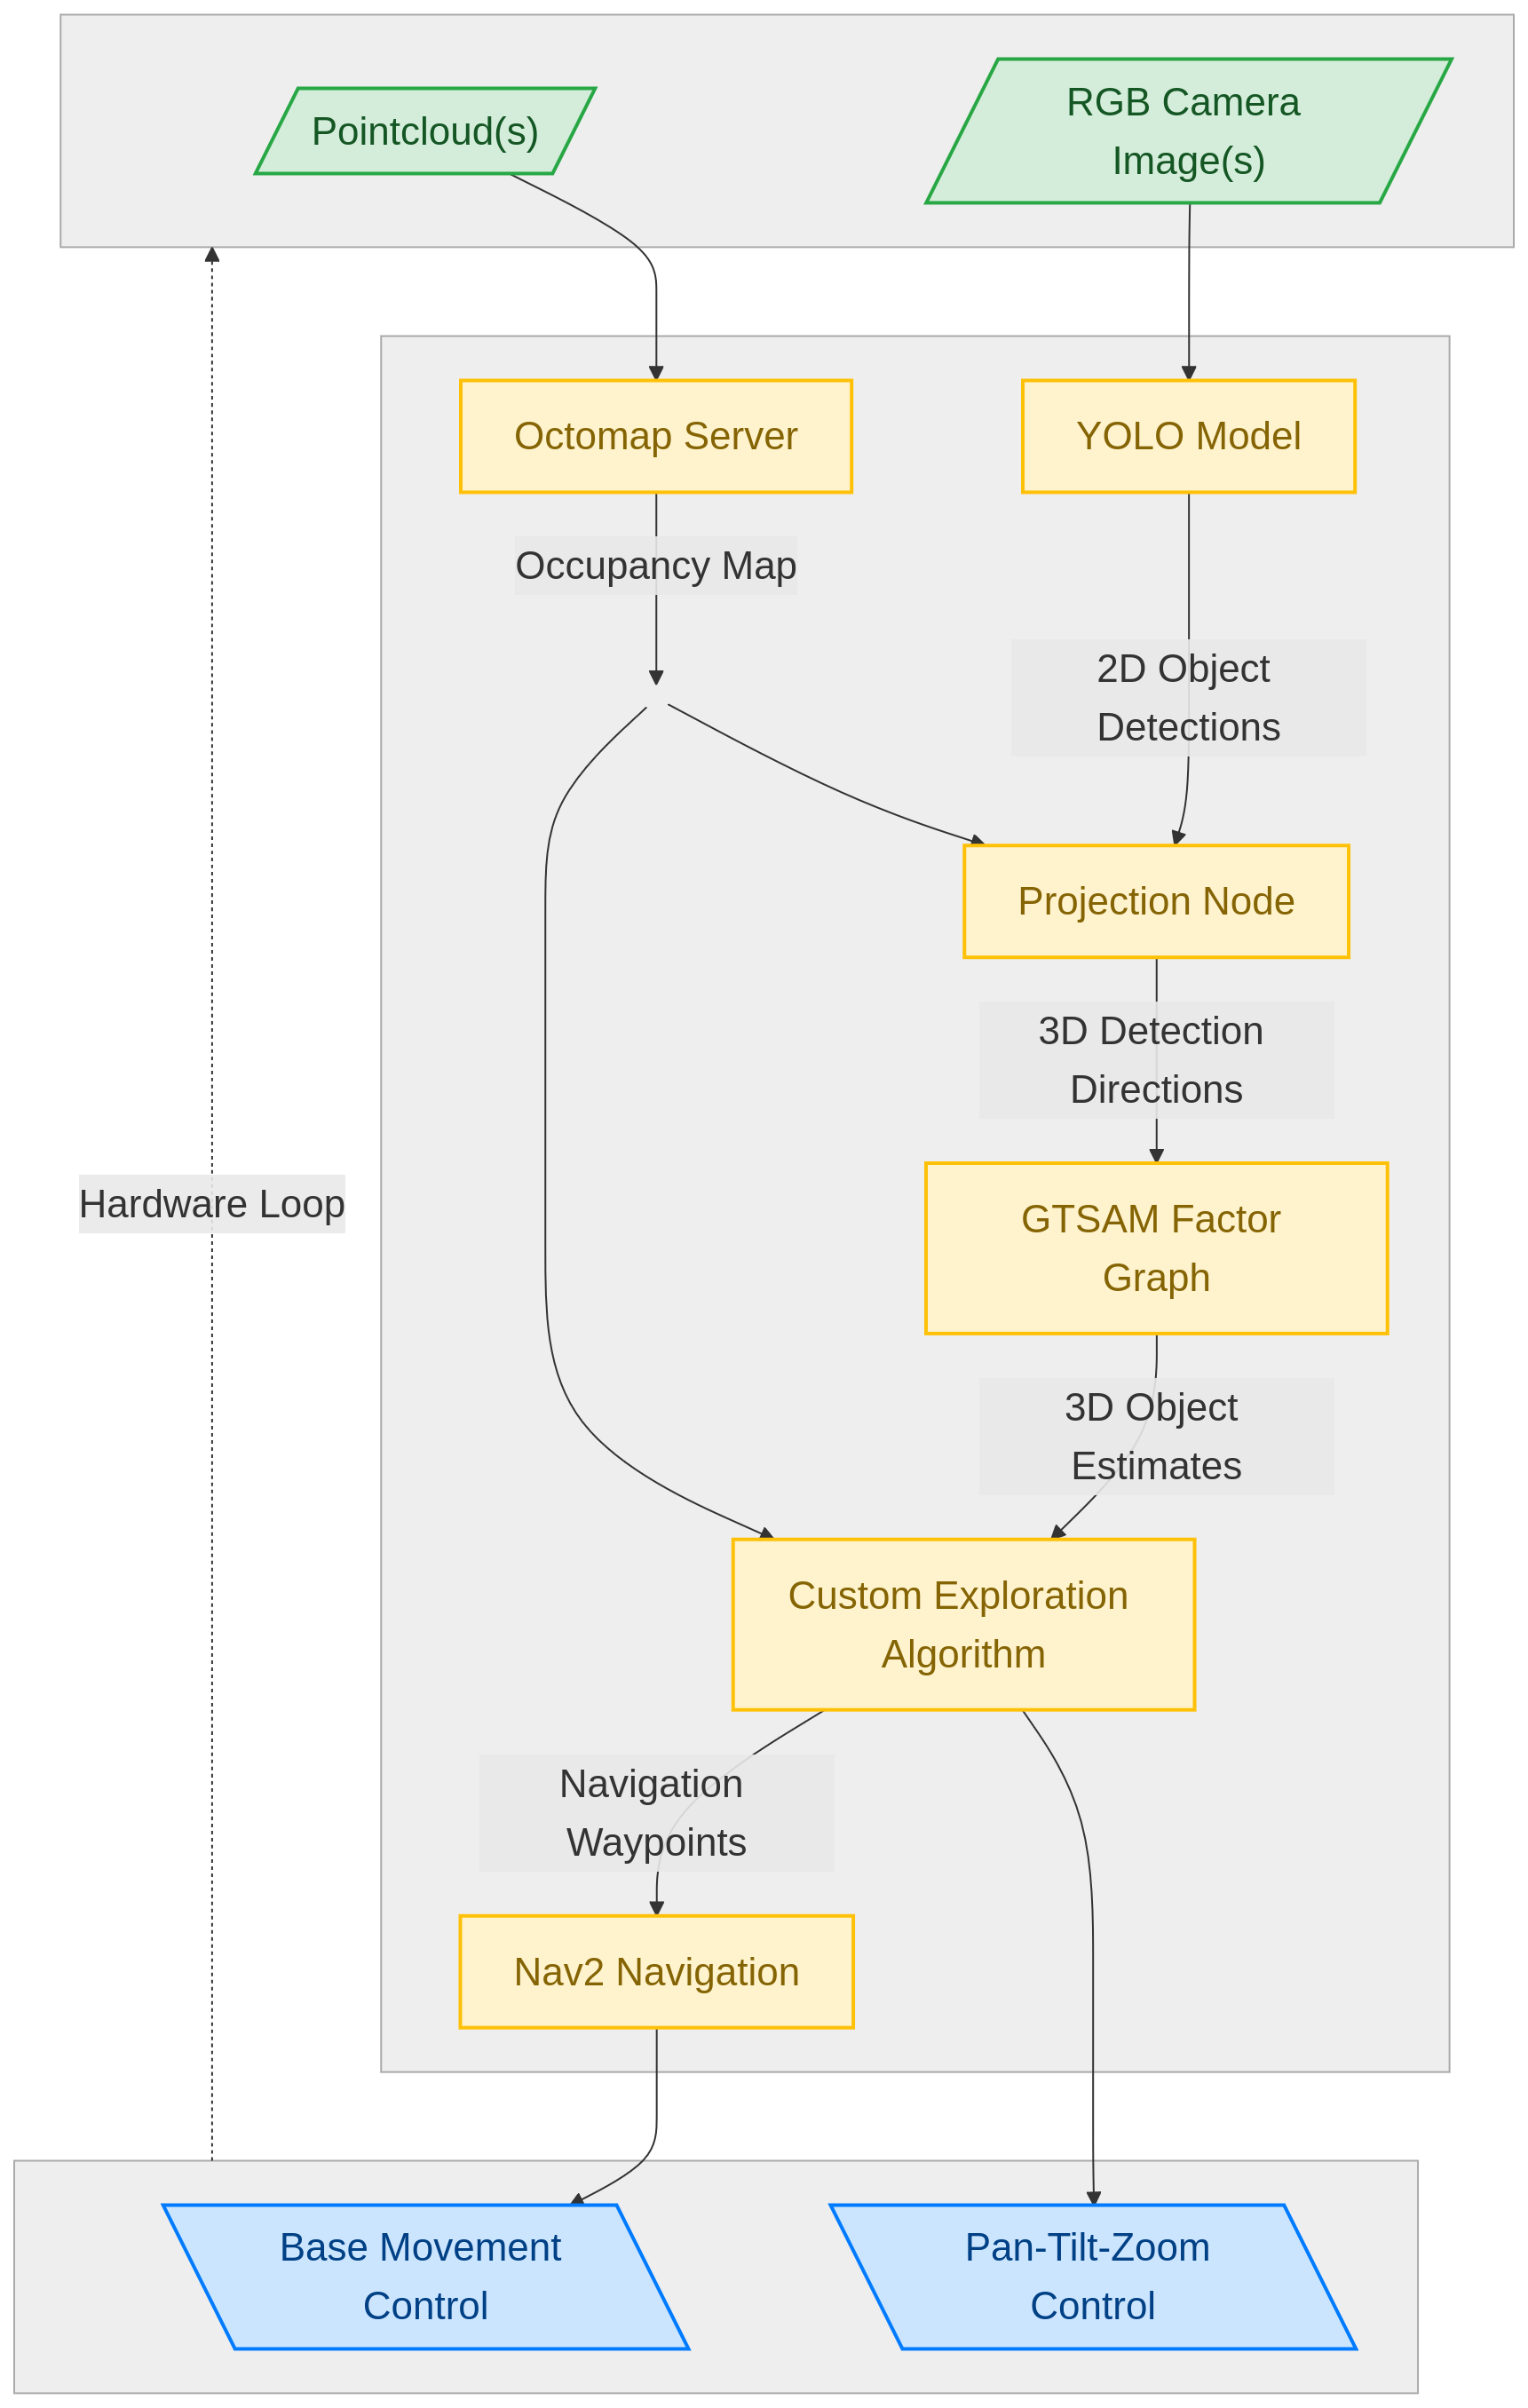
\includegraphics[width=0.75\textwidth]{assets/software_diagram.png}
    \caption{System architecture of the active visual search pipeline. Raw sensory inputs are processed through parallel mapping and object detection streams. The resulting 3D semantic estimates feed into the custom exploration algorithm, which closes the hardware loop by issuing decoupled commands to both the robot's base and the independent PTZ payload.}
    \label{fig:software_diagram}
\end{figure}

The software is fully implemented in ROS~2 \cite{robot_macenski_2022} and is highly adjustable via configuration files. This makes it possible to adapt the system to different robotic platforms and sensor configurations without requiring significant code changes. We demonstrate this configurability in detail by evaluating the final system with two different robots and environments, as presented in Chapter~\ref{ch:experiments}. The rest of this chapter focuses on the system specifications and methodology, independent of the platform used.

% %%{init: { 'themeVariables': { 'fontSize': '22px' } }}%%
% flowchart TD

%     %% Styling
%     classDef inputStyle fill:#d4edda,stroke:#28a745,stroke-width:2px,color:#155724
%     classDef outputStyle fill:#cce5ff,stroke:#007bff,stroke-width:2px,color:#004085
%     classDef moduleStyle fill:#fff3cd,stroke:#ffc107,stroke-width:2px,color:#856404
%     classDef moduleStyle fill:#fff3cd,stroke:#ffc107,stroke-width:2px,color:#856404
%     classDef invisibleStyle fill:none,stroke:none,color:none;

%     style IN fill:#eeeeee,stroke:#aaaaaa;
%     style OUT fill:#eeeeee,stroke:#aaaaaa;
%     style MODULES fill:#eeeeee,stroke:#aaaaaa;

%     %% Inputs
%     subgraph IN[ ]
%         IN_POINTS[/"Pointcloud(s)"/]:::inputStyle
%         IN_360[/"RGB Camera Image(s)"/]:::inputStyle
%     end

%     %% Modules
%     subgraph MODULES[ ]
%         MODULE_DETECTOR[YOLO Model]:::moduleStyle
%         MODULE_OPTIMIZER[GTSAM Factor Graph]:::moduleStyle
%         MODULE_OCOTMAP[Octomap Server]:::moduleStyle
%         MODULE_EXPLORER[Custom Exploration Algorithm]:::moduleStyle
%         MODULE_NAV2[Nav2 Navigation]:::moduleStyle
%         MODULE_PROJECTOR["Projection Node"]:::moduleStyle
%         INVISIBLE(( )):::invisibleStyle
%     end

%     %% Outputs
%     subgraph OUT[ ]
%         OUT_TWIST[\Base Movement Control\]:::outputStyle
%         OUT_PTZ[\Pan-Tilt-Zoom Control\]:::outputStyle
%     end

%     %% Input Connections
%     IN_POINTS --> MODULE_OCOTMAP
%     IN_360 --> MODULE_DETECTOR

%     %% Detector
%     MODULE_DETECTOR -- 2D Object Detections --> MODULE_PROJECTOR

%     MODULE_PROJECTOR -- 3D Detection Directions --> MODULE_OPTIMIZER

%     %% Optimizer
%     MODULE_OPTIMIZER -- 3D Object Estimates --> MODULE_EXPLORER
    
%     %% Octomap Server
%     MODULE_OCOTMAP -- Occupancy Map --> INVISIBLE
%     INVISIBLE --> MODULE_EXPLORER
%     INVISIBLE --> MODULE_PROJECTOR

%     %% Explorer
%     MODULE_EXPLORER -- Navigation Waypoints --> MODULE_NAV2
%     MODULE_EXPLORER --> OUT_PTZ

%     %% Nav 2
%     MODULE_NAV2 --> OUT_TWIST

%     %% Physical Loop
%     OUT -. "Hardware Loop".-> IN 
%     %% ROBOT((Robot)) -.-> IN
%     %%IN_POINTS ~~~ ROBOT

\section{Mapping}
By the nature of exploration algorithms, we assume the robot starts in an unknown environment and must build a map online to navigate. Conceptually, an occupancy map achieves this by chopping the continuous physical space into a grid of discrete voxels. Each voxel holds a probability score indicating whether that specific patch of space includes an obstacle, is completely clear, or still unobserved.

To construct this probabilistic 3D map in practice, we rely on the OctoMap library~\cite{hornung13auro}. Internally, OctoMap takes an incoming point cloud topic and stores its occupancy estimates inside an octree data structure, updating individual voxels incrementally as new sensor measurements arrive. This multi-resolution representation keeps memory usage highly efficient while allowing fast volumetric queries, such as casting rays through the map to determine object visibility or estimate 3D positions.

To handle base movement efficiently, the full 3D map is flattened into a lightweight 2D projected occupancy grid map. This 2D representation is ideal for standard path planning, obstacle avoidance, and frontier computation without the computational cost of processing the full 3D volume. Figure~\ref{fig:octomap} shows both the 3D representation and the resulting 2D projection of an example environment in our simulation.

\begin{figure}[h]
    \centering
    
    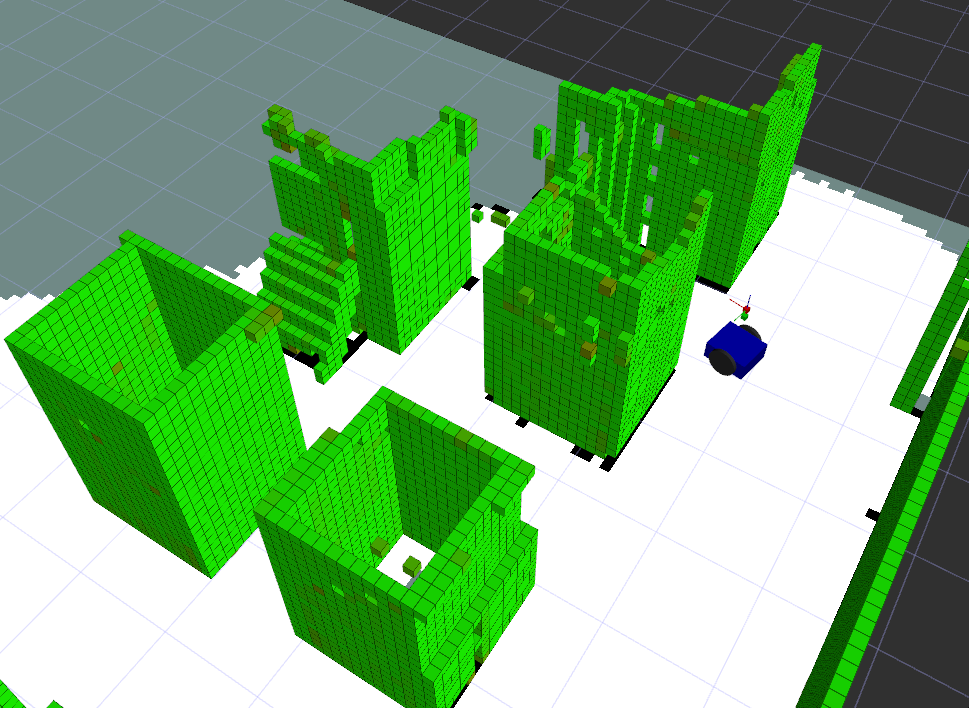
\includegraphics[width=0.48\linewidth, valign=m]{assets/octomap_3d.png}
    \hfill
    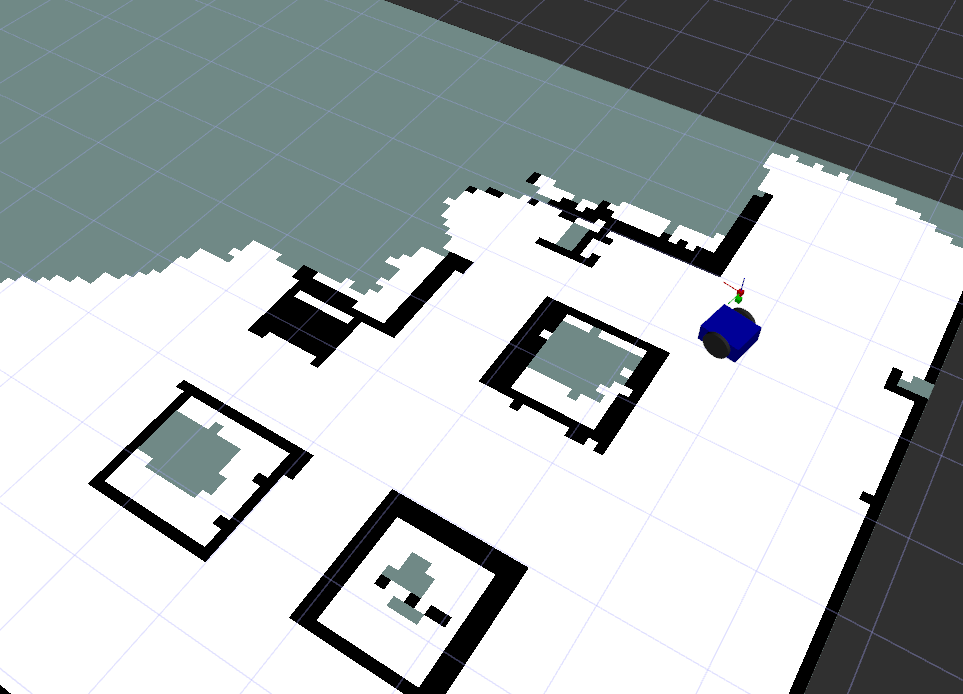
\includegraphics[width=0.48\linewidth, valign=m]{assets/octomap_2d.png}
    
    \par\vspace{5pt}
    
    \begin{subfigure}[t]{0.48\linewidth}
        \caption{3D occupancy grid map visualization}
    \end{subfigure}
    \hfill
    \begin{subfigure}[t]{0.48\linewidth}
        \caption{2D projected occupancy grid map}
    \end{subfigure}

    \caption{Representations of the simulated environment. The full 3D occupancy map (a) is used for volumetric reasoning, while its flattened 2D projection (b) provides a lightweight grid for efficient base navigation.}
    \label{fig:octomap}
\end{figure}

\section{Navigation}
To control the robot's base and reliably move it from one exploration waypoint to another, we utilize the highly modular Nav2 framework~\cite{macenski2020marathon2}. Our custom exploration node later acts as a client to Nav2 via a python interface. This allows the exploration module to asynchronously dispatch target poses, query path lengths to evaluate frontier candidates, and monitor task execution results directly within our high-level state machine.

% \afterpage{
%   \begin{figure}[H]
%     \begin{center}
%       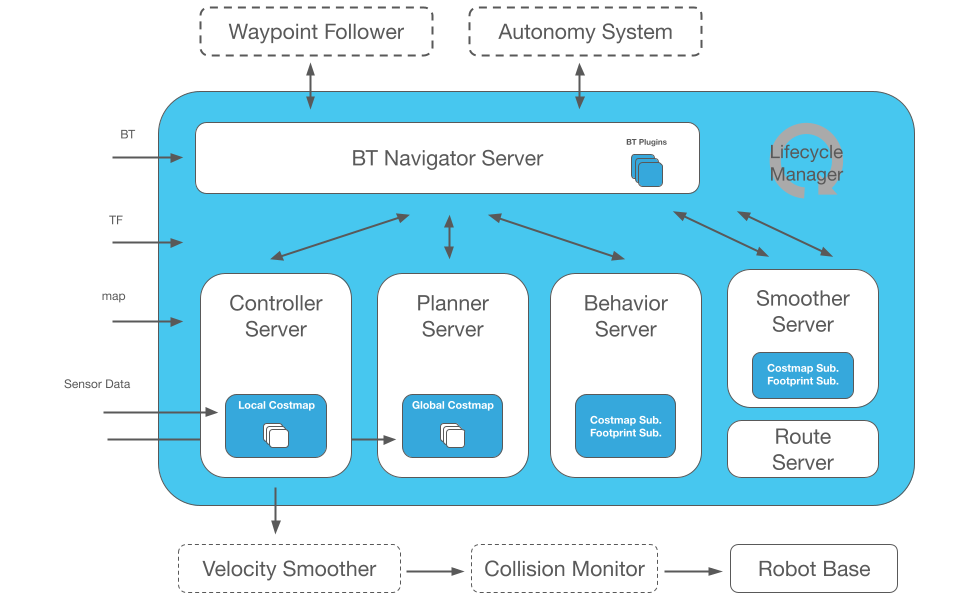
\includegraphics[width=1\linewidth]{assets/nav2_architecture.png}
%         \caption[Overview of the Nav2 package architecture]{Overview of the Nav2 package architecture. {\footnotemark}}
%     \label{fig:nav2}
%     \end{center}
%   \end{figure}
%   \footnotetext{Source: \url{https://docs.nav2.org/}}
% }

Our system treats navigation as a point-to-point transit mechanism. We implemented a custom behavior tree intentionally removing standard physical recovery behaviors (such as spinning in place or executing backup maneuvers). Instead, high-level failure handling is delegated entirely to our exploration module later. If a global path cannot be computed or the local controller fails to make progress, the navigation stack simply aborts the action and the exploration node will register and handle the failure by re-evaluating the next goal location.

Internally, the navigation task relies on a global planner to evaluate the flattened 2D occupancy grid map and a local controller to compute safe velocity commands. Because this chapter is designed to be generic, the underlying plugins and safety parameters can be freely adjusted to match the physical properties of the target platform. Transitioning from our simulated mobile base to the physical robot for example required swapping the local trajectory execution controller, updating the base footprint dimensions, adjusting costmap inflation layers, and mapping the coordinate transforms to the platform's native visual odometry frames. This structural flexibility ensures that the active search framework remains decoupled from the low-level kinematic constraints of any specific hardware platform.

\section{Object Detection}
In order for the robot to detect the desired objects, we rely on the widespread object detection framework YOLO~\cite{look_joseph_2016}. More specifically, we use the at the time newest official implementation of YOLO26n by Ultralytics~\cite{Jocher_Ultralytics_YOLO_2023}. YOLO is a simple yet effective one-pass object detection framework that is highly optimized for real-time inference, framing detection as a single regression problem to simultaneously predict bounding boxes and class probabilities across the entire image. The default YOLO model weights are trained on the Common Objects in Context (COCO) dataset~\cite{microsoft_lin_2014}, a large-scale benchmark containing over 80 object classes ranging from people and backpacks to various indoor furniture. We use those weights directly without any further training or fine-tuning.

Our implementation is designed to take an arbitrary number of camera streams as input and run detection efficiently on all of them. Each YOLO detection provides a semantic class label $c$, a confidence score $p$, and a 2D bounding box. We denote the bounding box $b$ by its center pixel $(u,v)$ and its width and height $(w,h)$ in pixels. At this stage, a raw detection is naturally represented as a tuple $d$ containing just the semantic and 2D spatial information:
\begin{align}
b &= (u, v, w, h),
& d &= (c, p, b)
\end{align}

\section{Detection Projection}
To utilize these 2D detections for 3D state estimation, we must project them into the physical environment. All detections of the desired classes are interpreted as a direction from the camera origin toward the bounding box center of the object, with a Gaussian uncertainty in the bearing angle. Figure~\ref{fig:detections} shows a 2D YOLO detection and how it is interpreted as a bearing in 3D space.

\begin{figure}[h]
    \centering
    
    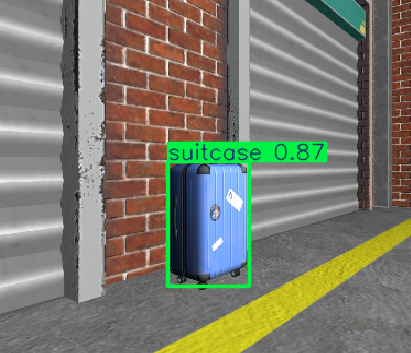
\includegraphics[width=0.48\linewidth, valign=m]{assets/detection.png}
    \hfill
    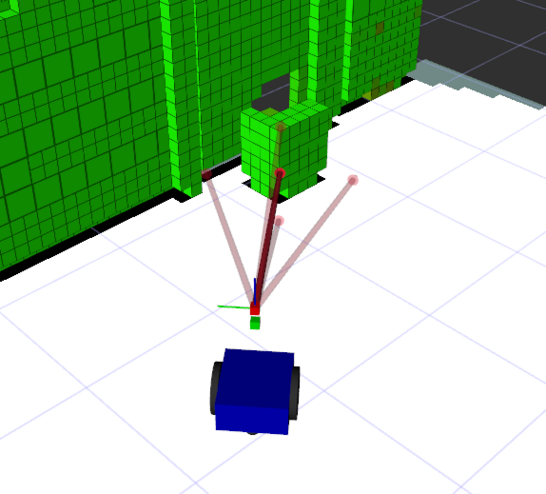
\includegraphics[width=0.48\linewidth, valign=m]{assets/detection_direction.png}
    
    \par\vspace{5pt}
    
    \begin{subfigure}[t]{0.48\linewidth}
        \caption{YOLO detection in the 2D image}
    \end{subfigure}
    \hfill
    \begin{subfigure}[t]{0.48\linewidth}
        \caption{Detection visualized in 3D world}
    \end{subfigure}

    \caption{Projection of a 2D object detection into 3D coordinates. The bounding box from the 2D camera feed (a) is transformed into a 3D bearing measurement (b). The solid red arrow represents the nominal ray cast from the camera origin to the first occupied voxel in the environment. The four faded arrows outline the uncertainty cone. Scaled by a 2D $\chi^2$ confidence interval, these vectors visualize the statistical region ($95\%$ probability) where the object's true center is expected to lie, derived from the bearing standard deviations.}
    \label{fig:detections}
\end{figure}

For later fusion, we expand the raw detection into a measurement tuple $z$, containing the semantic information alongside the 3D bearing measurement, its angular uncertainty, and an optional range measurement:
\begin{align}
z &= (c, p, \alpha, \beta, \sigma_{\alpha}, \sigma_{\beta}, [r, \sigma_{r}]),
\end{align}

where the bracketed elements denote the optional range $r$ and its associated uncertainty $\sigma_{r}$, which are only present if depth information is available.

Let $(f_x,f_y,c_x,c_y)$ be the camera intrinsics obtained from the ROS~2 camera info topic. We first convert the pixel center $(u,v)$ into normalized image coordinates $(x,y)$:
\begin{align}
x &= \frac{u - c_x}{f_x},
& y &= \frac{v - c_y}{f_y}
\end{align}

Using the pinhole model, the corresponding unit-length bearing vector in the camera frame $C$ is
\begin{align}
\mathbf{r}_C &= \frac{1}{\sqrt{x^2 + y^2 + 1}}\begin{bmatrix}x\\y\\1\end{bmatrix}.
\end{align}

To express the ray in the global world frame $W$, we take the rigid transform from camera to world at the detection timestamp, consisting of a rotation $\mathbf{R}_{WC}\in SO(3)$ and translation $\mathbf{t}_{WC}\in\mathbb{R}^3$. This yields the world-frame ray direction $\mathbf{r}_W$ and camera origin $\mathbf{o}_W$; the full ray is parameterized by $\lambda\ge 0$:
\begin{align}
\mathbf{r}_W &= \mathbf{R}_{WC}\,\mathbf{r}_C,
& \mathbf{o}_W &= \mathbf{t}_{WC},
& \mathbf{p}_W(\lambda) &= \mathbf{o}_W + \lambda\,\mathbf{r}_W.
\end{align}

Once the continuous ray $\mathbf{p}_W(\lambda)$ is defined in the world frame, we cast it through the 3D occupancy map built by OctoMap. We search for the first occupied voxel in that direction that corresponds to the detected object. If an occupied voxel is hit within a maximum valid ray distance, we establish a range measurement $r = \lambda_{hit}$ corresponding to the distance from the camera origin to the object's surface. If no obstacle is hit, the detection remains a bearing-only measurement.

We describe the bearing by azimuth $\alpha$ and elevation $\beta$ defined in the camera frame:
\begin{align}
\alpha &= \operatorname{atan2}(r_{C,x}, r_{C,z}),
& \beta &= \operatorname{atan2}(r_{C,y}, \sqrt{r_{C,x}^2 + r_{C,z}^2}).
\end{align}

Finally, we formulate heuristic models to estimate the measurement uncertainties. These models rely on tunable parameters that we have adjusted for our application. The bearing uncertainty we approximate from the bounding box size. Intuitively, larger boxes tend to have less reliable centers. We model the unknown true pixel center as a Gaussian perturbation around the reported center, with standard deviations $\sigma_u = m\,w/4$ and $\sigma_v = m\,h/4$, where $m$ is a tuneable parameter and $(w, h)$ are the bounding box dimensions. With this choice, the $\pm 2\sigma$ interval corresponds to a horizontal band of total width $m\,w$ around the reported center (and a vertical band of total height $m\,h$), which contains approximately $95\%$ of the probability mass for a 1D Gaussian. Tuning $m$ directly adjusts the percentage of the bounding box extent that we ``trust'' to contain the true center with high probability (per axis). We then convert the pixel uncertainty to an angular uncertainty via the focal length and add a minimum noise floor $\sigma_{bearing\_min}$ (in radians). 
\begin{align}
\sigma_{\alpha} &= \sqrt{\left(\frac{m\,w}{4 f_x}\right)^2 + \sigma_{bearing\_min}^2} \\
\sigma_{\beta} &= \sqrt{\left(\frac{m\,h}{4 f_y}\right)^2 + \sigma_{bearing\_min}^2}
\end{align}

If the ray casting successfully returned a range measurement $r$, we also compute a range uncertainty. We use a proportional error model assuming that the uncertainty grows linearly with the measured distance, combined with a minimum range noise floor $\sigma_{r,\min}$ (in meters) to account for the spatial discretization of the Octomap voxels. For this we introduce another tunable parameter $k$ as the range multiplier.
\begin{align}
\sigma_{r} &= \sqrt{\left(k \, r\right)^2 + \sigma_{r,\min}^2}
\end{align}

\section{Object Location Estimation}
In order to infer the 3D position of target objects, detections first need to be associated correctly with previously seen instances and then combined into a consistent 3D estimate. In this work, the physical target objects detected by the vision system are modeled mathematically as \textit{landmarks} within the factor graph architecture. For this, we rely on factor graph optimization.

\subsection{Data Association}

In order to fuse detections over time, each new measurement must be associated with either an already confirmed landmark, a candidate landmark, or stored temporarily until a new landmark can be initialized. This process follows a pipeline that prioritizes high-confidence matches while maintaining flexibility for ambiguous detections.

As described previously, each detection is represented as a bearing measurement and its associated Gaussian uncertainty, optionally accompanied by range. Regardless of whether a range measurement is available, we exclusively use the bearing components for the initial data association process to maintain dimensional consistency across all observations. For association, we use the azimuth-elevation representation $\mathbf{y} = [\alpha,\beta]^\top$ with measurement covariance
\begin{align}
\mathbf{R}_{meas} = \begin{bmatrix}
\sigma_{\alpha}^2 & 0 \\
0 & \sigma_{\beta}^2
\end{bmatrix},
\end{align}
where $(\sigma_{\alpha},\sigma_{\beta})$ are derived from the detected bounding box size as described in the previous section.

\textbf{Overall Pipeline.} The data association process operates in three stages, outlined in Pseudocode~\ref{alg:overall_pipeline}. First, all incoming measurements are matched against confirmed landmarks $L_{conf}$. Any unpaired measurements are then compared against candidate landmarks $L_{cand}$ which act as a buffer for ambiguous or weakly supported objects. Finally, measurements still remaining are either triangulated into new candidates or stored in a pending buffer $Z_{pend}$ for future association. Paired measurements are immediately integrated into the factor graph, while candidates are promoted to confirmed landmarks only after receiving sufficient repeated support.

\begin{algorithm}[h]
\caption{Overall Detection Association Pipeline} 
\label{alg:overall_pipeline} 
\textbf{Input:} New measurements $Z$, Confirmed Landmarks $L_{conf}$, Candidate Landmarks $L_{cand}$, Pending Measurements $Z_{pend}$ \\
\textbf{Output:} Updated $L_{conf}$, $L_{cand}$, and $Z_{pend}$
\begin{algorithmic}[1]
    \State \textit{// Stage 1: Match against Confirmed Landmarks}
    \State Paired$_{conf}$, Unpaired $\leftarrow$ \Call{ICNN}{$Z$, $L_{conf}$}
    \State Update $L_{conf}$ with Paired$_{conf}$ and add to factor graph
    
    \If{Unpaired $\neq \emptyset$}
        \State \textit{// Stage 2: Match remaining against Candidate Landmarks}
        \State Paired$_{cand}$, Still\_Unpaired $\leftarrow$ \Call{ICNN}{Unpaired, $L_{cand}$}
        
        \State \textit{// Stage 3: Manage Candidates (Promotion \& Triangulation)}
        \State \Call{Manage\_Candidates}{Paired$_{cand}$, Still\_Unpaired, $L_{cand}$, $Z_{pend}$, $L_{conf}$}
    \EndIf
\end{algorithmic}
\end{algorithm}

\textbf{Individually Compatible Nearest Neighbor (ICNN)} Both stages 1 and 2 rely on the ICNN algorithm \cite{data_neira_2001} which is described in Pseudocode~\ref{alg:icnn}. This algorithm matches each measurement to the closest landmark if one exists within a statistical gate. The greedy nature of ICNN makes it computationally efficient, and the staged approach ensures that confirmed landmarks are matched before candidates.

\begin{algorithm}[h]
\caption{ICNN with Chi-square Gating} 
\label{alg:icnn} 
\textbf{Funct} \Call{ICNN}{$Z$, $L$}
\begin{algorithmic}[1]
    \State Paired $\leftarrow \emptyset$, Unpaired $\leftarrow \emptyset$
    \For{\textbf{each} measurement $z_i \in Z$}
        \State $min\_dist \leftarrow \infty$
        \State $best\_match \leftarrow null$
        
        \For{\textbf{each} landmark $l_j \in L$}
            \State $D^2 \leftarrow$ MahalanobisDistance($z_i$, $l_j$)
            \If{$D^2 \leq \chi^2_{2, \alpha_{gate}}$ \textbf{and} $D^2 < min\_dist$}
                \State $min\_dist \leftarrow D^2$
                \State $best\_match \leftarrow l_j$
            \EndIf
        \EndFor
        
        \If{$best\_match \neq null$}
            \State Paired $\leftarrow$ Paired $\cup \{ (z_i, best\_match) \}$
        \Else
            \State Unpaired $\leftarrow$ Unpaired $\cup \{ z_i \}$
        \EndIf
    \EndFor
    \State \textbf{return} Paired, Unpaired
\end{algorithmic}
\end{algorithm}

The core of the matching step is computing a statistical compatibility score between each measurement and landmark. For each landmark $l_j$, we predict the expected bearing $\hat{\mathbf{y}}_j$ in the current camera frame by projecting the landmark estimate using the corresponding TF transform at the detection timestamp. We then compute the squared Mahalanobis distance between the expected $\hat{\mathbf{y}}_j$ and actual measurement $\mathbf{y}_j$:
\begin{align}
D^2(\mathbf{y},l_j) &= (\mathbf{y}-\hat{\mathbf{y}}_j)^\top\, \mathbf{S}^{-1}\, (\mathbf{y}-\hat{\mathbf{y}}_j),
\end{align}
where the covariance matrix $\mathbf{S}$ combines measurement and prediction uncertainties:
\begin{align}
\mathbf{S} &= \mathbf{R}_{meas} + \mathbf{R}_{pred}(l_j).
\end{align}
Here, $\mathbf{R}_{meas}$ is the measurement covariance from the detection, and $\mathbf{R}_{pred}(l_j)$ is the predicted bearing covariance induced by the landmark's current 3D uncertainty and camera pose. This yields a statistically meaningful compatibility score in units of standard deviations.

To determine if a measurement-landmark pair is compatible, we perform a chi-square hypothesis test with significance level $\alpha_{gate}$. A pair is accepted if
\begin{align}
D^2 \leq \chi^2_{2,\alpha_{gate}},
\end{align}
where the two degrees of freedom correspond to the two bearing angles $(\alpha,\beta)$. Among all compatible landmarks, Algorithm~\ref{alg:icnn} selects the one with the smallest $D^2$.

\begin{algorithm}[h]
\caption{Candidate Promotion and Triangulation} 
\label{alg:manage_candidates} 
\textbf{Funct} \Call{Manage\_Candidates}{Paired$_{cand}$, Unpaired, $L_{cand}$, $Z_{pend}$, $L_{conf}$}
\begin{algorithmic}[1]
    \State \textit{// Part I: Promote supported candidates}
    \For{\textbf{each} $(z_i, c_j) \in$ Paired$_{cand}$}
        \State $c_j.support \leftarrow c_j.support + 1$
        \If{$c_j.support \geq$ \textsc{Promotion\_Threshold}}
            \State Move $c_j$ from $L_{cand}$ to $L_{conf}$
            \State Initialize $c_j$ in factor graph
        \EndIf
    \EndFor
    
    \State \textit{// Part II: Triangulate remaining unpaired measurements}
    \For{\textbf{each} $z_u \in$ Unpaired}
		\State $min\_ray\_distance \leftarrow \infty$
        \State $best\_candidate\_point \leftarrow null$
        \State $best\_pending\_measurement \leftarrow null$
        \For{\textbf{each} $z_p \in Z_{pend}$}
            \State ray\_distance, point\_3d $\leftarrow$ \Call{Triangulate}{$z_u, z_p$}
            
            \If{ray\_distance $<$ \textsc{Max\_Intersection\_Error} \\ \quad \quad \quad  \textbf{and} ray\_distance $<$ min\_ray\_distance}
                \State $min\_ray\_distance \leftarrow$ ray\_distance
                \State $best\_candidate\_point \leftarrow$ point\_3d
                \State $best\_pending\_measurement \leftarrow z_p$
            \EndIf
        \EndFor
        
        \If{$best\_candidate\_point \neq null$}
			\State $candidate \leftarrow$ \Call{Create\_Candidate}{best\_candidate\_point, $z_u.class$}
			\State Add $candidate$ to $L_{cand}$
			\State Remove $best\_pending\_measurement$ from $Z_{pend}$
        \Else
            \State Add $z_u$ to $Z_{pend}$ \textit{// Save for future triangulation}
        \EndIf
    \EndFor
\end{algorithmic}
\end{algorithm}

\textbf{Candidate Management and Triangulation.} Measurements that remain unpaired after matching against both confirmed and candidate landmarks enter the candidate management stage as seen in Pseudocode~\ref{alg:manage_candidates}. Candidates are promoted to confirmed landmarks once they receive sufficient repeated support from multiple observations. This two-stage commitment process prevents spurious detections or misclassifications from polluting the confirmed set.

For unpaired measurements, the system attempts to triangulate them with observations from a pending buffer $Z_{pend}$. Each unpaired measurement $z_u$ is paired with each pending measurement $z_p$, and a 3D candidate point is computed from the ray intersection. If the ray intersection error is below a threshold, a new candidate landmark is created and added to $L_{cand}$. Otherwise, the measurement is stored in $Z_{pend}$ for later triangulation with future observations.

\subsection{Factor Graph Optimization}
We estimate landmark positions using factor graph optimization. A factor graph is a bipartite graph consisting of variable nodes (unknown states) and factor nodes (probabilistic constraints) that jointly define a posterior over all variables. In our case, the variables are landmark positions, while factors encode prior camera pose information and bearing measurements. Solving the graph corresponds to a nonlinear least-squares optimization that yields the maximum a posteriori (MAP) estimate. A resulting factor graph plotted on a projected 2D plane can be seen in Figure~\ref{fig:gtsam}.

\begin{figure}[h]
    \centering
    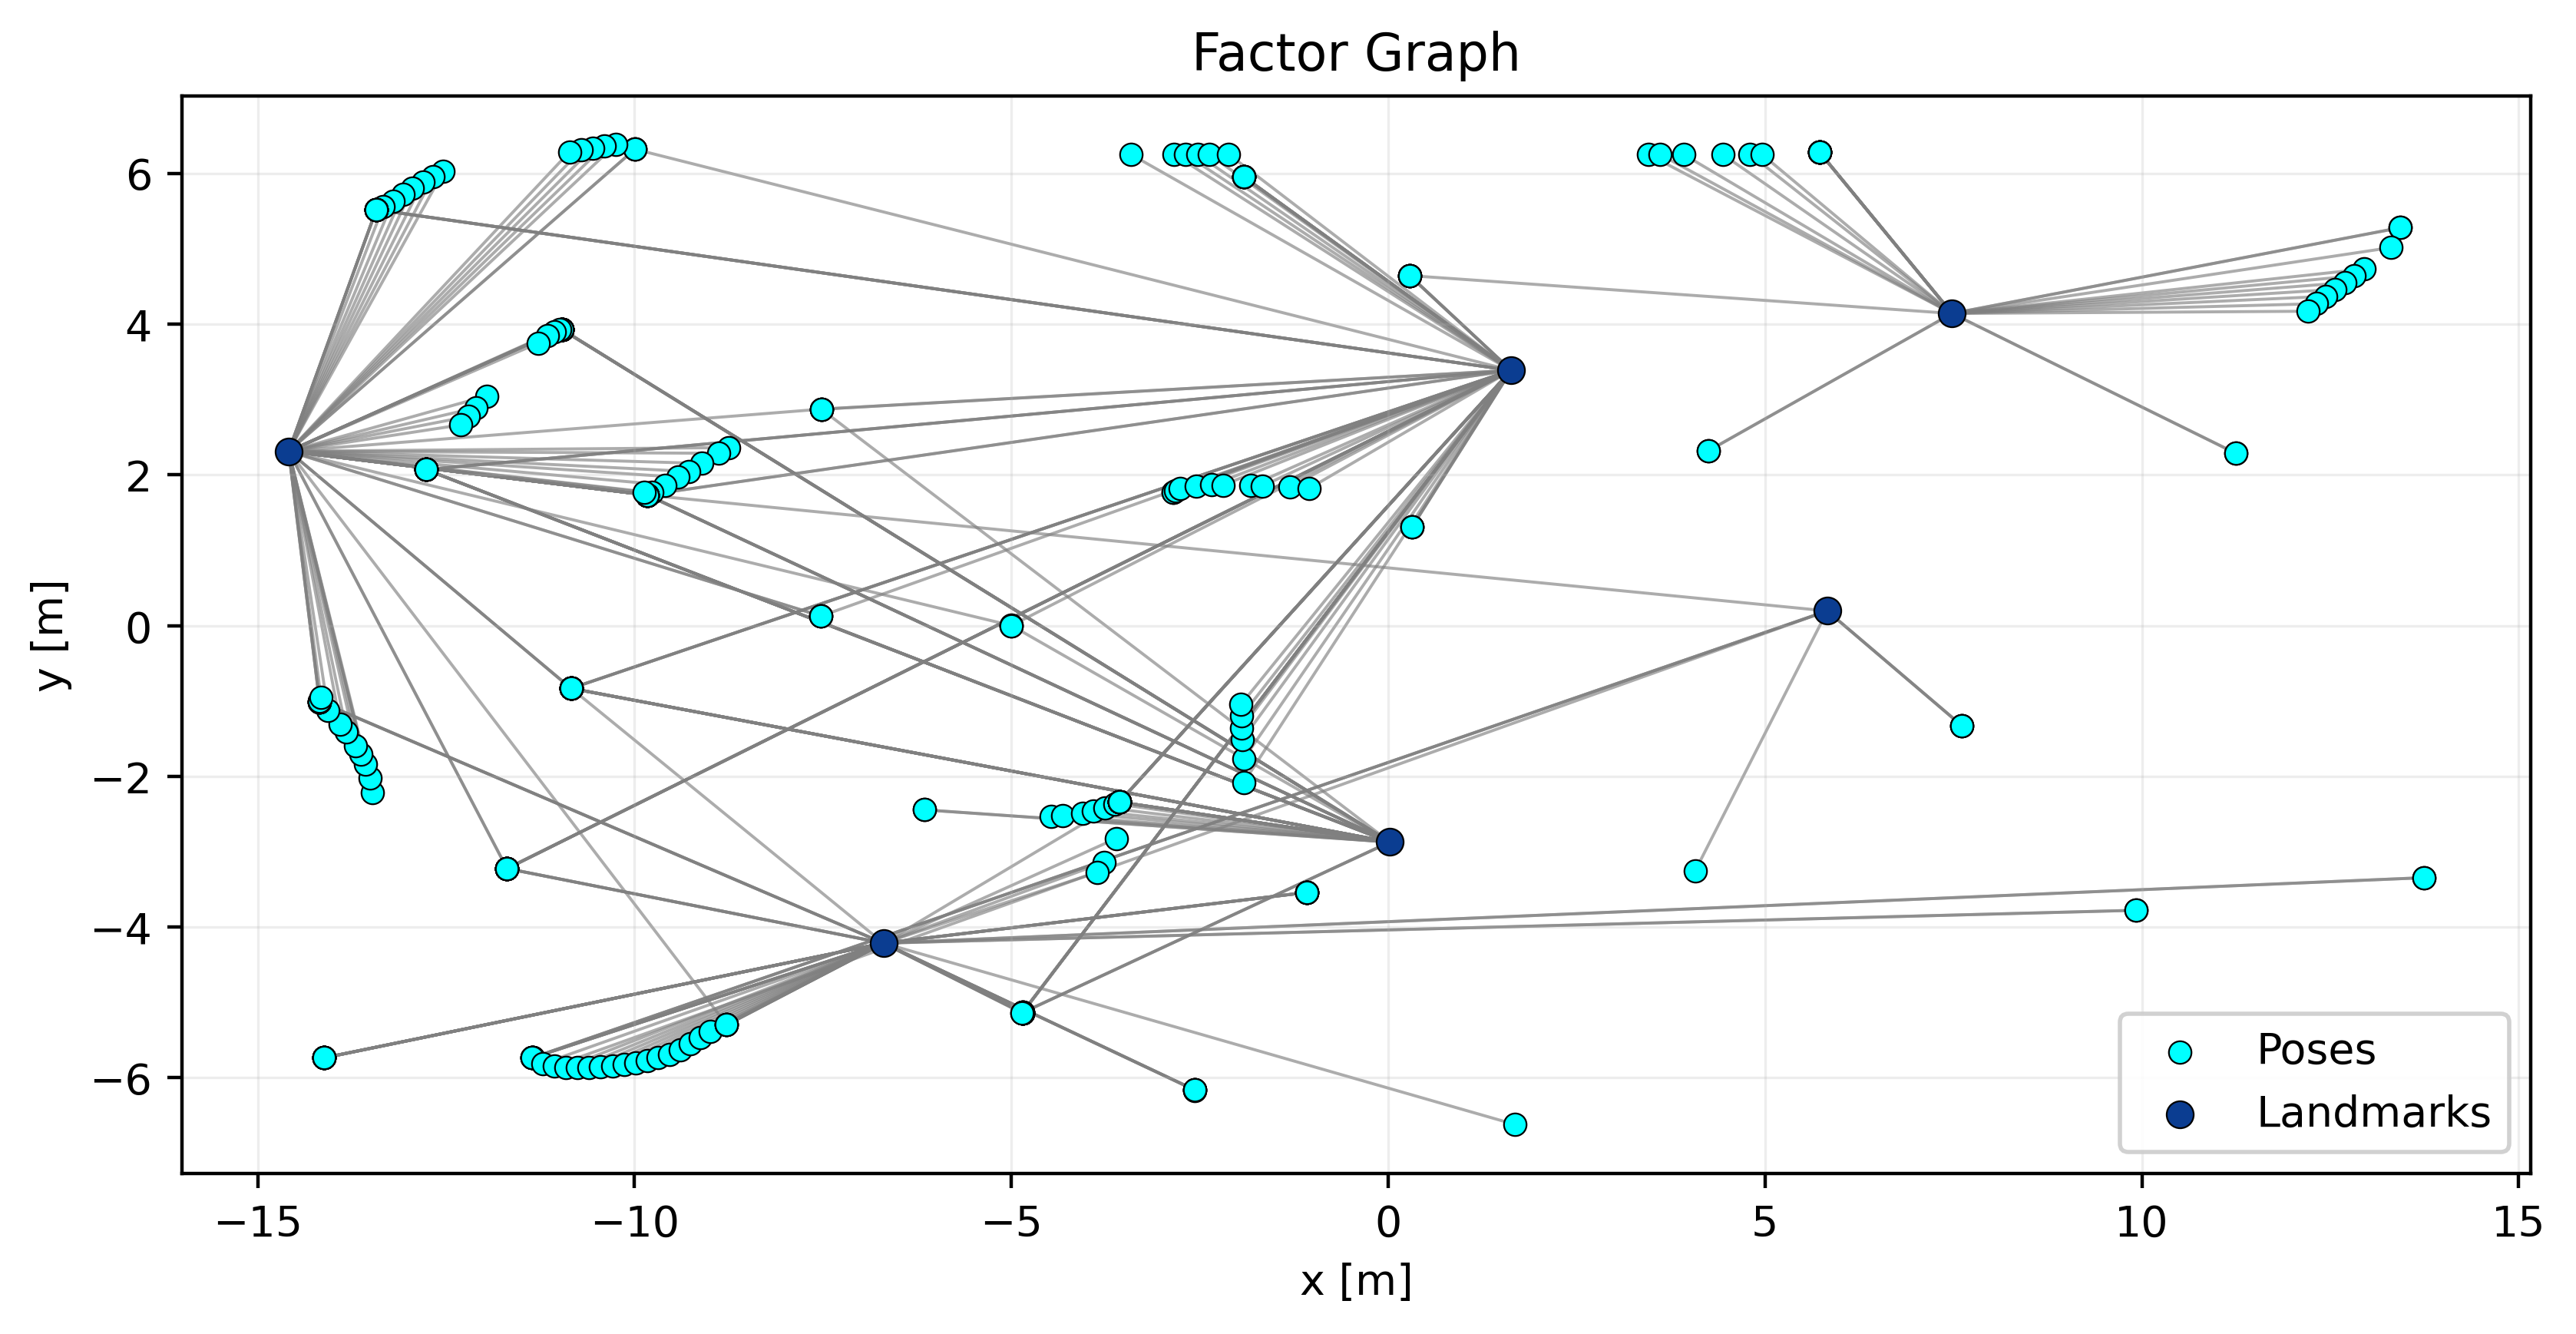
\includegraphics[width=0.95\textwidth]{assets/factor_graph.png}
    \caption{A top-down 2D projection of the optimized factor graph after full exploration of an environment with six target objects. The bipartite structure consists of variable nodes representing camera poses (light circles) and landmark positions (dark circles). The connecting edges visualize the network of observation factors that constrain the landmarks relative to the robot's trajectory.}
    \label{fig:gtsam}
\end{figure}

All measurements that were associated with confirmed landmarks are added as observation factors to the graph, using their measurement covariances as noise models. The type of factor added depends directly on the available data from the detection projection step. If the measurement contains only bearing information, it is added as a \texttt{BearingFactor}. If the measurement also includes range data (from a successful OctoMap ray intersection), it is integrated using a joint \texttt{BearingRangeFactor}. This flexibility ensures that we can extract the maximum possible constraint information from depth measurements without strictly requiring them. For each measurement batch, we also add a pose prior for the camera pose node with a tight uncertainty. Because we rely on the highly robust navigation stack of the robot (such as Boston Dynamics Spot), we confidently treat the camera poses as securely fixed relative to the world frame by anchoring them with these tight priors, rather than chaining them sequentially with complex robot odometry factors.

To prevent the graph from growing unbounded with redundant data, we filter incoming measurements before they are evaluated. Observations are discarded if the camera has not moved a sufficient translational or rotational distance since the last update, or if they arrive too closely in time. However, this pose-based gating is explicitly bypassed if a change in the PTZ camera's zoom (focal length) is detected. Enhancing the focal length provides new, localized high-resolution information even from a standstill, thereby justifying the addition of new measurement factors.

The factor graph is maintained and optimized using the GTSAM library~\cite{gtsam}, specifically employing iSAM2~\cite{isam2_kaess_2012}. Instead of resolving the entire graph from scratch during every cycle, iSAM2 performs incremental nonlinear optimization. It achieves real-time performance by updating a Bayes tree representation and only relinearizing variables whose estimates have changed beyond a configurable threshold. 

This optimization step intrinsically supports our data association pipeline. After each optimization cycle, we extract the updated 3D marginal covariance for each confirmed landmark. This tight, newly optimized uncertainty is then fed back into the subsequent timestep's ICNN matching gate. This establishes a continuous loop where better position estimates directly produce more accurate statistical gating limits, leading to cleaner and more robust data association overall.

\section{Exploration and Object Search}
With the mapping, navigation and detection pipeline in place we can now define the exploration and object search methodology. We chose to implement a simple frontier exploration algorithm, loosely following the publication of Yamauchi et. al~\cite{frontierbased_yamauchi_1997}. We also define three different PTZ control maneuvers to integrate active search into the pipeline.

\subsection{Frontier Computation}
To select the next goal point the robot should travel to in order to efficiently explore the map we use the projected map of the occupancy gridmap provided by the Octomap Server. Relying on the 2D information alone is sufficient since we assume a planar world with one floor only. For this we continuously scan the most recent received 2D projected occupancy map for frontiers.

Formally, let $O(i,j) \in \{\text{free}, \text{occupied}, \text{unknown}\}$ denote the occupancy value of grid cell $(i,j)$. A cell is considered a frontier if:
\begin{align}
	(i,j) \in F \iff O(i,j) = \text{free} \; \wedge \; \exists (i',j') \in N_8(i,j): O(i',j') = \text{unknown},
\end{align}
where $N_8(i,j)$ denotes the eight-connected neighborhood. Figure~\ref{fig:frontiers} shows an example gridmap to visualize the concept of frontiers.

\begin{figure}[h]
    \centering
    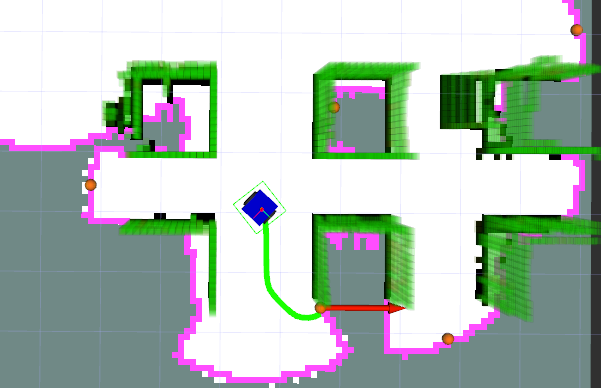
\includegraphics[width=0.75\textwidth]{assets/frontiers.png}
    \caption{Visualization of frontier detection and clustering on a projected 2D occupancy grid. Purple cells denote the continuous boundary regions where known free space directly borders unexplored areas. These raw frontier cells are grouped via 8-connectivity, and each resulting cluster is assigned a single representative goal point (orange spheres) used for scoring and navigation.}
    \label{fig:frontiers}
\end{figure}

After the whole map has been classified into frontier and non-frontier cells, the frontiers are clustered using a simple connectivity check: any continuously connected region of frontier cells (using 8-connectivity) is called a frontier cluster. For each cluster, we compute a representative point by selecting the cell closest to the cluster's centroid:
\begin{align}
	r_k = \operatorname{argmin}_{p \in C_k} \|p - \operatorname{centroid}(C_k)\|_2,
\end{align}
where $C_k$ is the set of cells in cluster $k$ and $r_k$ is the representative cell. This representative point is then converted to world coordinates and scored in the next step.

\subsection{Goal Selection}
The score of each frontier cluster is computed as a weighted combination of two normalized features: the number of frontier cells and the distance between the robot and the frontier. For cluster $k$, let $s_k = |C_k|$ denote the cluster size (number of cells) and $d_k$ denote the distance from the robot to the cluster's representative point $r_k$ (either Euclidean distance or Nav2 path length, configurable). These are normalized per batch as:
\begin{align}
	\tilde{s}_k &= \frac{s_k}{\max_j s_j}, \quad \tilde{d}_k = 1 - \frac{d_k}{\max_j d_j}.
\end{align}
The final score is the weighted sum of the normalized features:
\begin{align}
	S_k = w_s \cdot \tilde{s}_k + w_d \cdot \tilde{d}_k,
\end{align}
where $w_s$ and $w_d$ are user-configurable weights that balance cluster size against proximity. Clusters are then ranked by score in descending order.

Goal selection proceeds as follows: frontiers are filtered to exclude any within a configurable blacklist radius of previously failed goals, and any closer to the robot than a minimum goal distance. From the remaining valid frontiers, the exploration node greedily selects the frontier with the highest score $S_k$ as the next navigation goal. This simple greedy approach prioritizes nearby, well-defined frontier clusters over distant or ambiguous ones.

With that done, the robot's basic geometric exploration algorithm is well defined. In order to include PTZ camera control in the exploration pipeline, we still need to control the PTZ cameras gaze to aid in object search. 

\subsection{PTZ Control}
For the evaluation we use three simple PTZ gaze maneuvers.

\begin{description}
    \item[Constant:] The PTZ camera remains fixed at a single default orientation. This serves as a passive baseline and does not actively adapt the camera view.

    \item[360-degree scan:] The camera is rotated through a full sweep in order to inspect the surrounding scene and increase the chance of observing new objects from multiple angles.

    \item[Landmark confirmation:] The current object hypotheses are first checked against the 3D scene geometry by projecting a ray from the camera into the occupancy map to verify that the object should be visible from the current pose. The PTZ camera is then aimed to look straight at the objects currents estimate. If no confident detection is obtained at the default 1x zoom setting, a short zoom ladder is used as an initial probing step to trigger a first detection. 
    Once the object has been detected, the camera then increases the zoom as much as possible while still keeping the object inside the field of view. Let $\phi_h(z)$ and $\phi_v(z)$ denote the horizontal and vertical field-of-view angles at zoom level $z$, and let $\alpha_o$ and $\beta_o$ denote the detection's angular half-width and half-height. The selected confirmation zoom $z^{\ast}$ is then
    \begin{align}
        z^{\ast} = \max \bigl\{ z_i \;\bigm|\; \phi_h(z_i) \ge 2(\alpha_o + \delta) \;\wedge\; \phi_v(z_i) \ge 2(\beta_o + \delta) \bigr\},
    \end{align}
    where $\delta$ is a small safety margin that prevents the target object from leaving the image during motion or calibration error. The gaze is kept for 4 seconds in order to allow the detection model to report the new observation successfully and afterwards the associated landmark is confirmed.
\end{description}

As we will see in the next chapters, these three maneuvers are progressively combined, to provide a simple benchmark from passive viewing to active gaze control and are used to compare the effect of PTZ support on object search performance.

\chapter{Experiments}
\label{ch:experiments}

To evaluate the developed system experiments were conducted both in a real world scenario as well as in a simulation. This chapter explains in detail the platforms and software used and the experiment setup for both environments.

\section{Real World Setup}
The main focus of the thesis was to develop and validate an active visual search system for the Spot robot. While the software architecture (see Section~\ref{sec:software}) is designed to be hardware-agnostic, this specific platform serves as our primary testbed to evaluate the framework's performance under actual kinematic and sensory constraints.

\subsection{Boston Dynamics Spot}

% Figure~\ref{fig:spot}:
\begin{figure}[h]
	\centering
	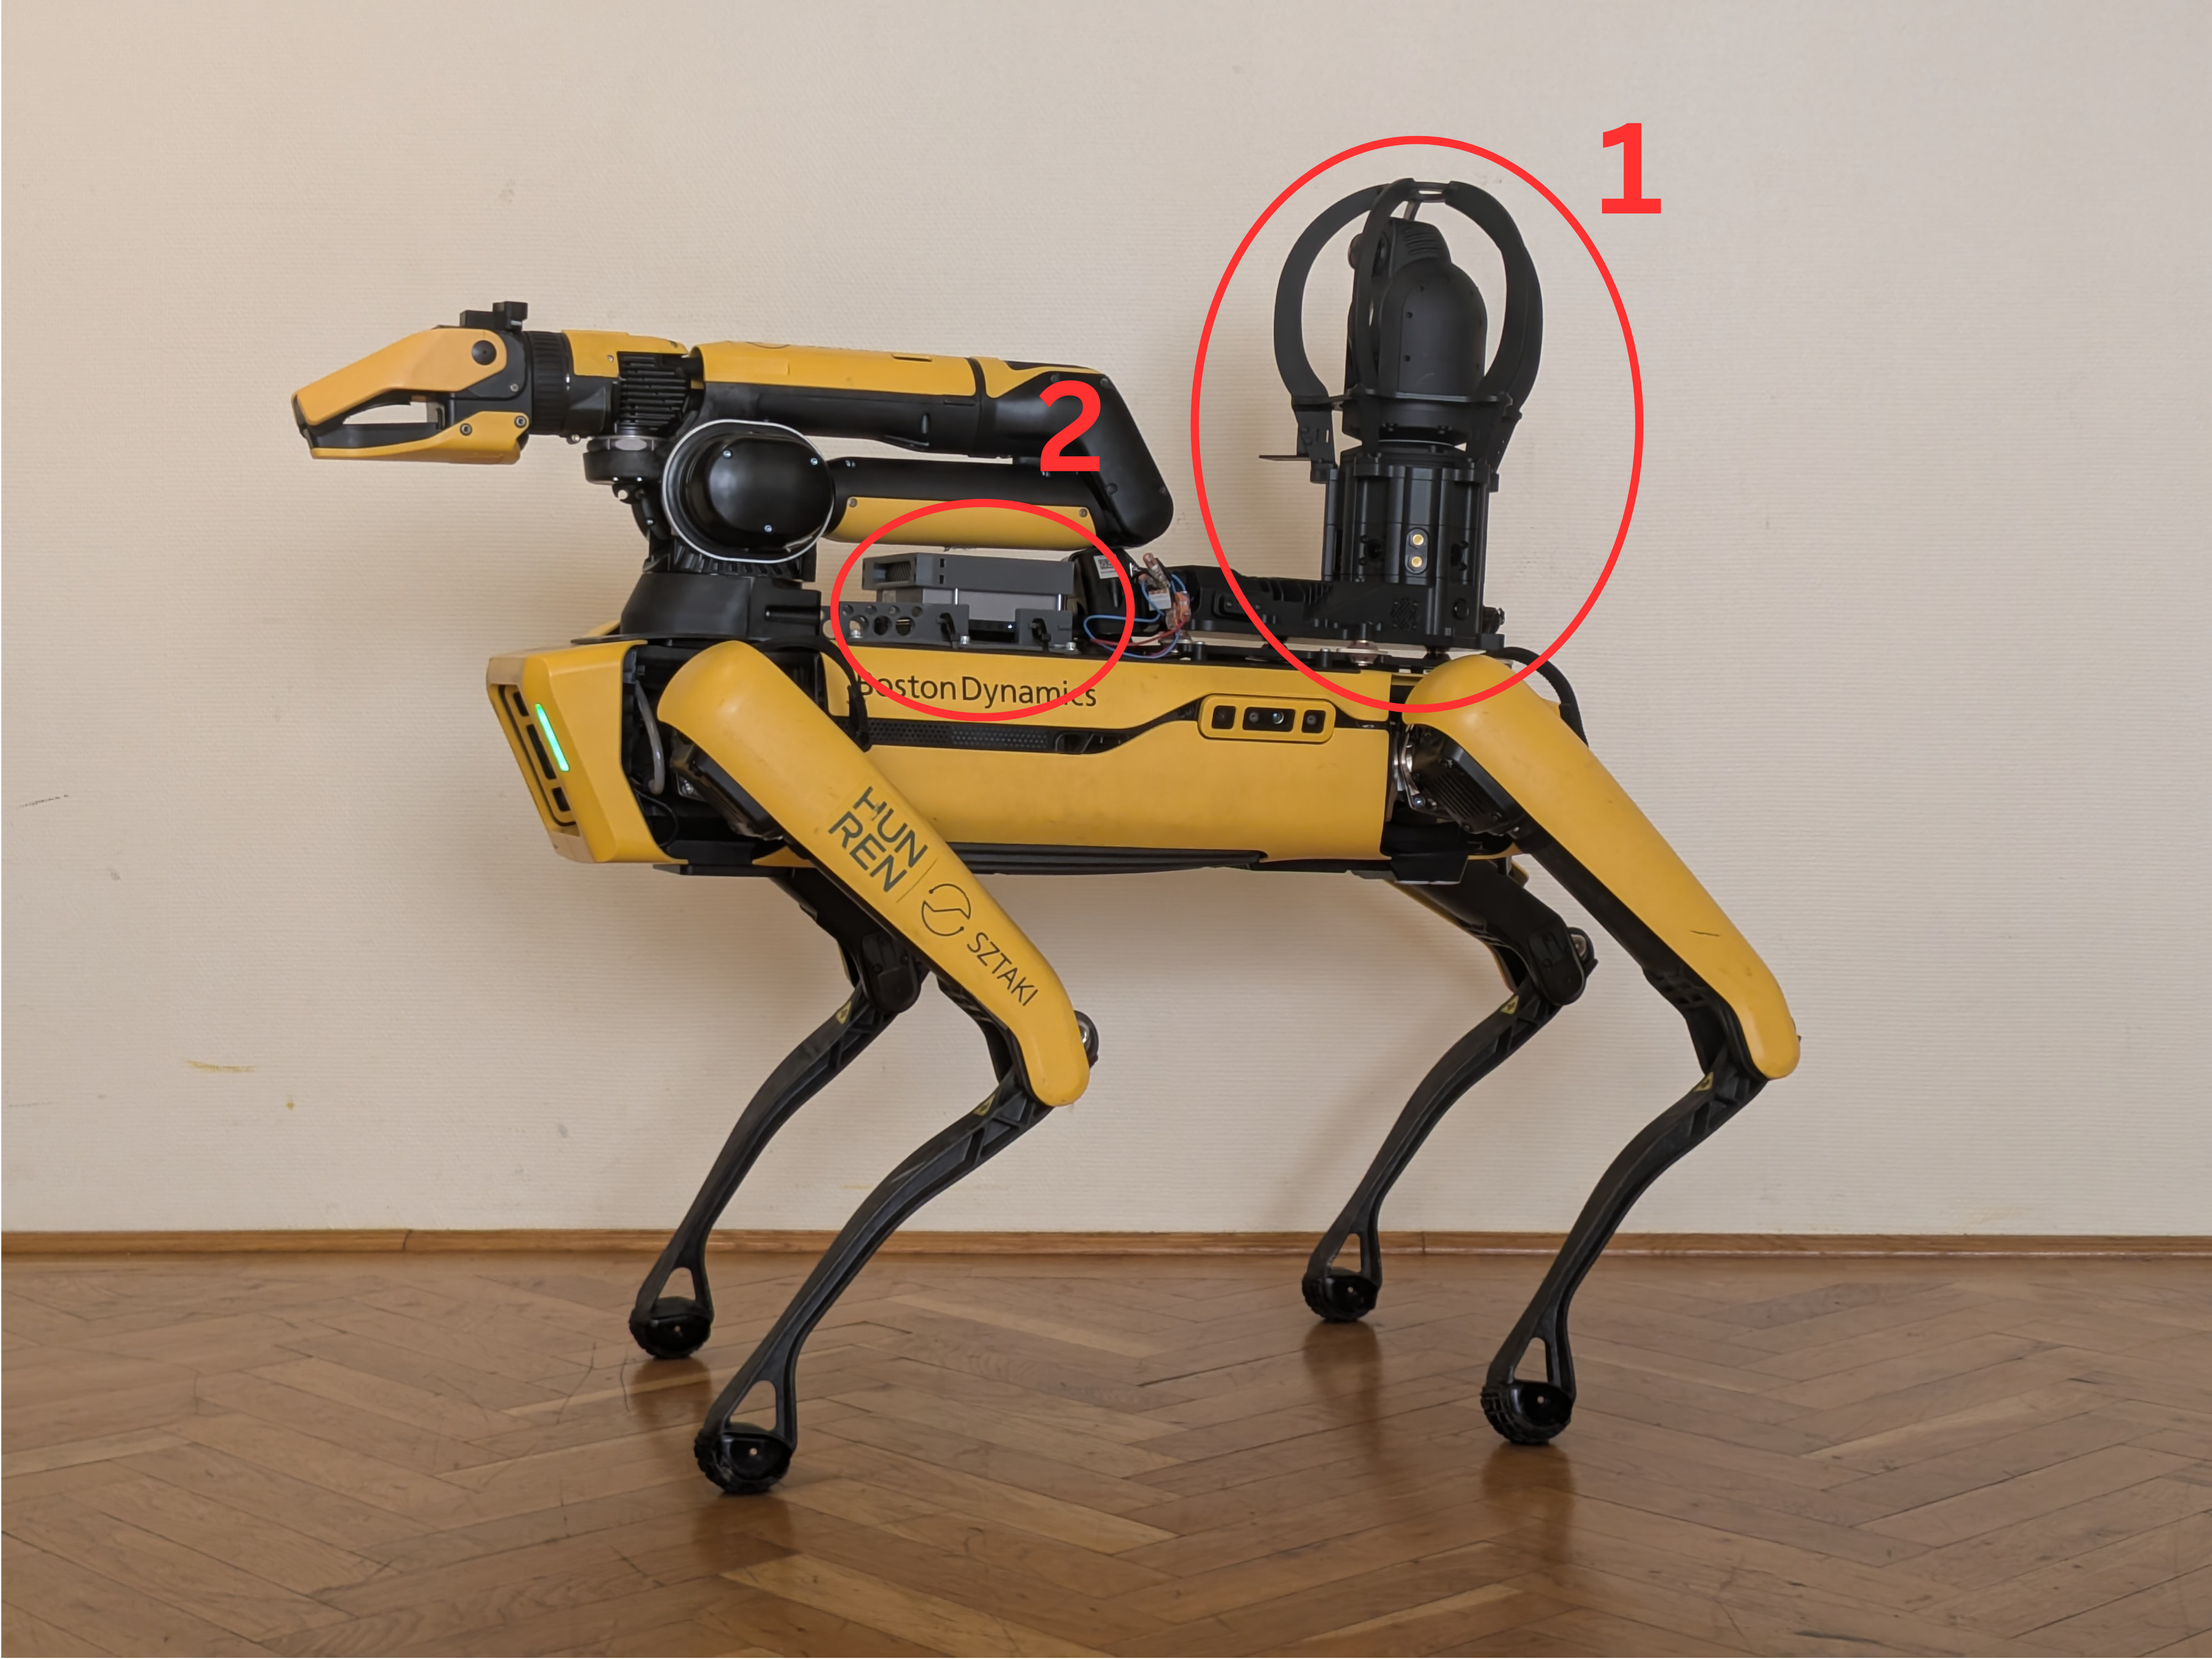
\includegraphics[width=0.8\textwidth]{assets/spot_scribbled.png}
	\caption{The Boston Dynamics Spot robot outfitted for active visual search. The annotations denote (1) the active PTZ payload and (2) the onboard NVIDIA Jetson Orin.}
    \label{fig:spot}
\end{figure}

\subsubsection{Hardware}
The hardware can be seen in Figure~\ref{fig:spot}. It consists of the legged mobile platform together with the official "SPOT Cam+ IR" payload\footnote{\url{https://support.bostondynamics.com/s/article/Spot-Cam-Setup-and-Usage-72060}} mounted on the lower back of the robot. This payload includes a PTZ camera whose RGB stream is used as the sole visual input for the object detection pipeline in the final experimental setup.
As the name suggests the payload also features an infrared camera as well as an array of five fisheye cameras that are stitched together providing a 360\textdegree{} view around the robot. For our purposes these were not used at all.

The robot itself has five RGB-D cameras integrated into its body that provide both color and depth images. We extract the depth information from these body cameras, aggregating it to serve as the unified input point cloud required by our mapping server.

Also mounted on the back of the robot is an NVIDIA Jetson Orin\footnote{\url{https://www.nvidia.com/en-us/autonomous-machines/embedded-systems/jetson-orin/}} computation unit that is directly connected to the robot via Ethernet. The Jetson Orin executes all necessary ROS~2 nodes locally, including the real-time YOLO26n object detection pipeline.

Finally, the robot features a robotic arm mounted on the front equipped with an additional RGB-D camera. For this project, we did not leverage the arm or its associated camera, always keeping the manipulator in the "stowed" position as seen in Figure~\ref{fig:spot}.

\subsubsection{Software}
The proprietary code running on the robots internal compute unit for localization, control and sensing is not modifiable. There is, however, a Python SDK\footnote{\url{https://dev.bostondynamics.com/readme}} available to interact with it over WiFi or ethernet. This allows reading the sensor signals and issuing commands for controlling the platform. Since our system is developed in ROS~2, we also use the \textit{spot\_ros2}\footnote{\url{https://github.com/rai-opensource/spot\_ros2}} package collection, which expose most of the Python SDK's API to ROS~2 topics, services, and actions. These packages also manage Spot's lease, publish standard ROS images and camera info topics, and handle the kinematic tree transformations (TF) of the robots joints. 

\begin{figure}[h]
	\centering
	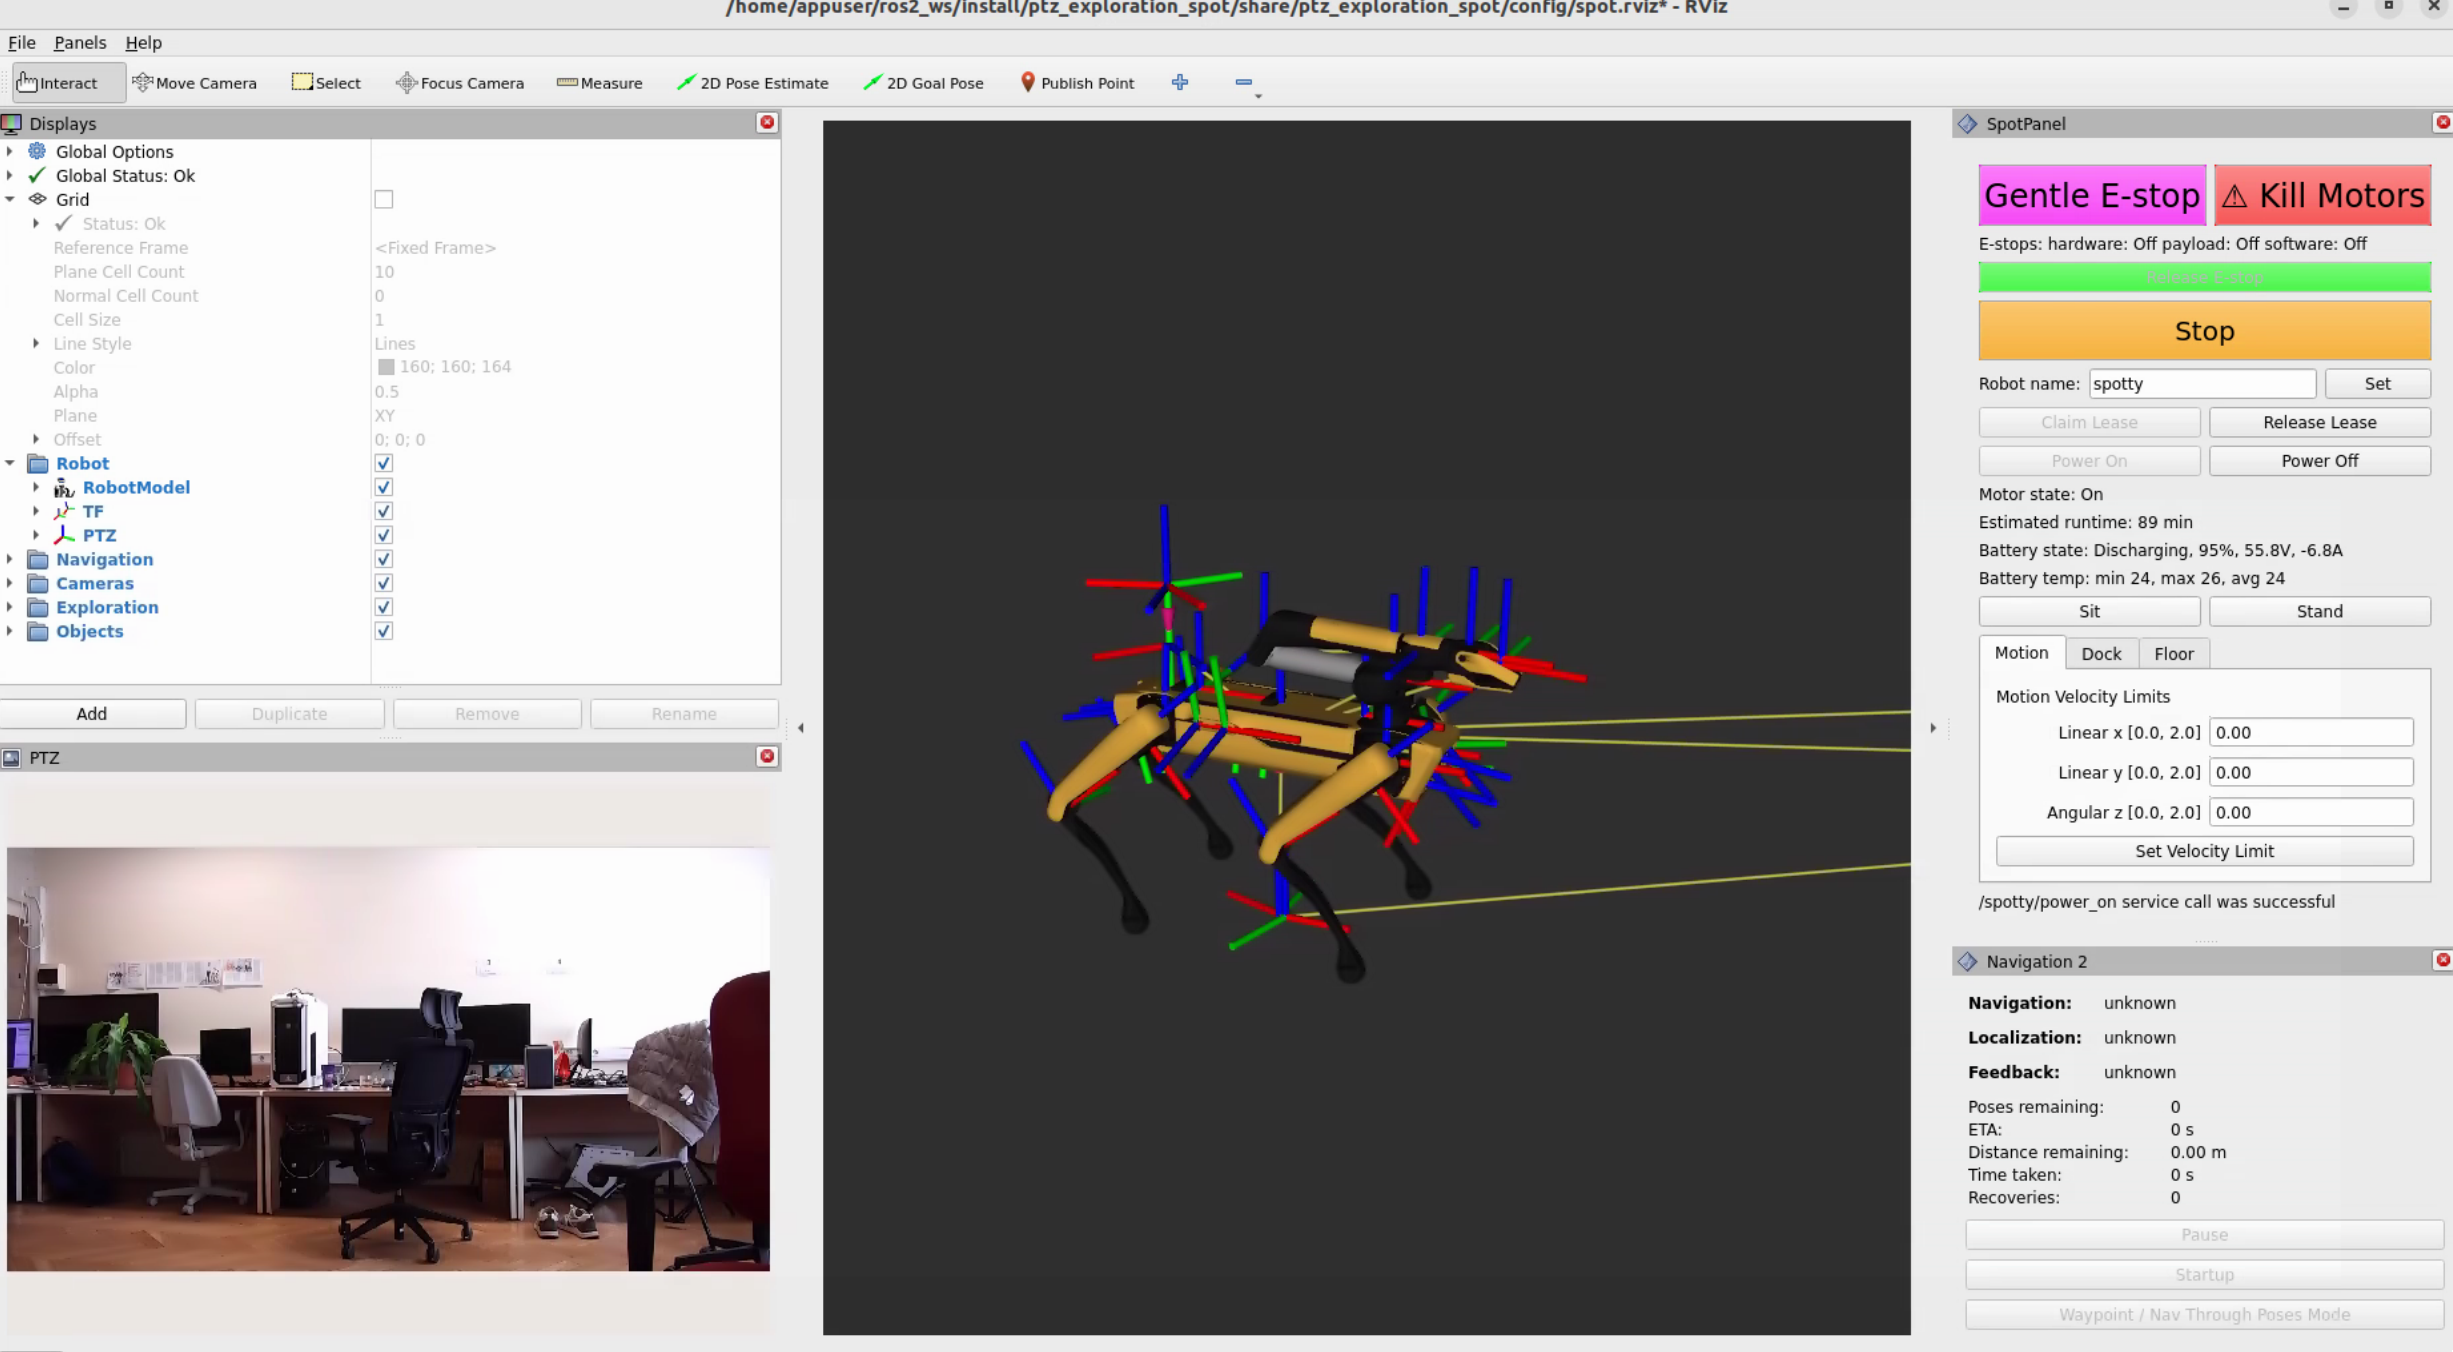
\includegraphics[width=1\textwidth]{assets/spot_rviz.png}
	\caption{RViz visualization interface used during physical deployment. The central view displays the robot's kinematic coordinate frames (TF tree), while the bottom-left panel confirms the integration of our custom driver by displaying the live PTZ video feed. The right panel features the \textit{spot\_ros2} dashboard for managing hardware leases and monitoring the robot's state.}
    \label{fig:spot_rviz}
\end{figure}

Because the "SPOT Cam+ IR" payload does not integrate seamlessly out-of-the-box with the \textit{spot\_ros2} packages we bridge this gap with a custom package, specifically developed as part of this thesis. This custom package is used to properly interface with the payload, forwarding commands (e.g., pan and tilt offsets), publishing the camera stream and info as ROS~2 topics and accurately maintaining payload TF frames and connecting them with the Spot's coordinate tree. Figure~\ref{fig:spot_rviz} shows RViz\footnote{\url{https://github.com/ros2/rviz}}, the standard 3D visualization environment for ROS, featuring the robot's model with all coordinate frames, as well as the camera view in the lower left corner.

\subsection{Environment and Target Objects}
The physical experiments were conducted in an office environment. We chose potted plants as the target object for the real-world search since they naturally occur in offices and directly correspond to the ``potted plant'' class in the standard COCO dataset. Figure~\ref{fig:plant_detections} shows a view inside this office environment. The evaluation environment consists of one big room and a hallway, with a total of four plants for the robot to discover.

\begin{figure}[h]
	\centering
	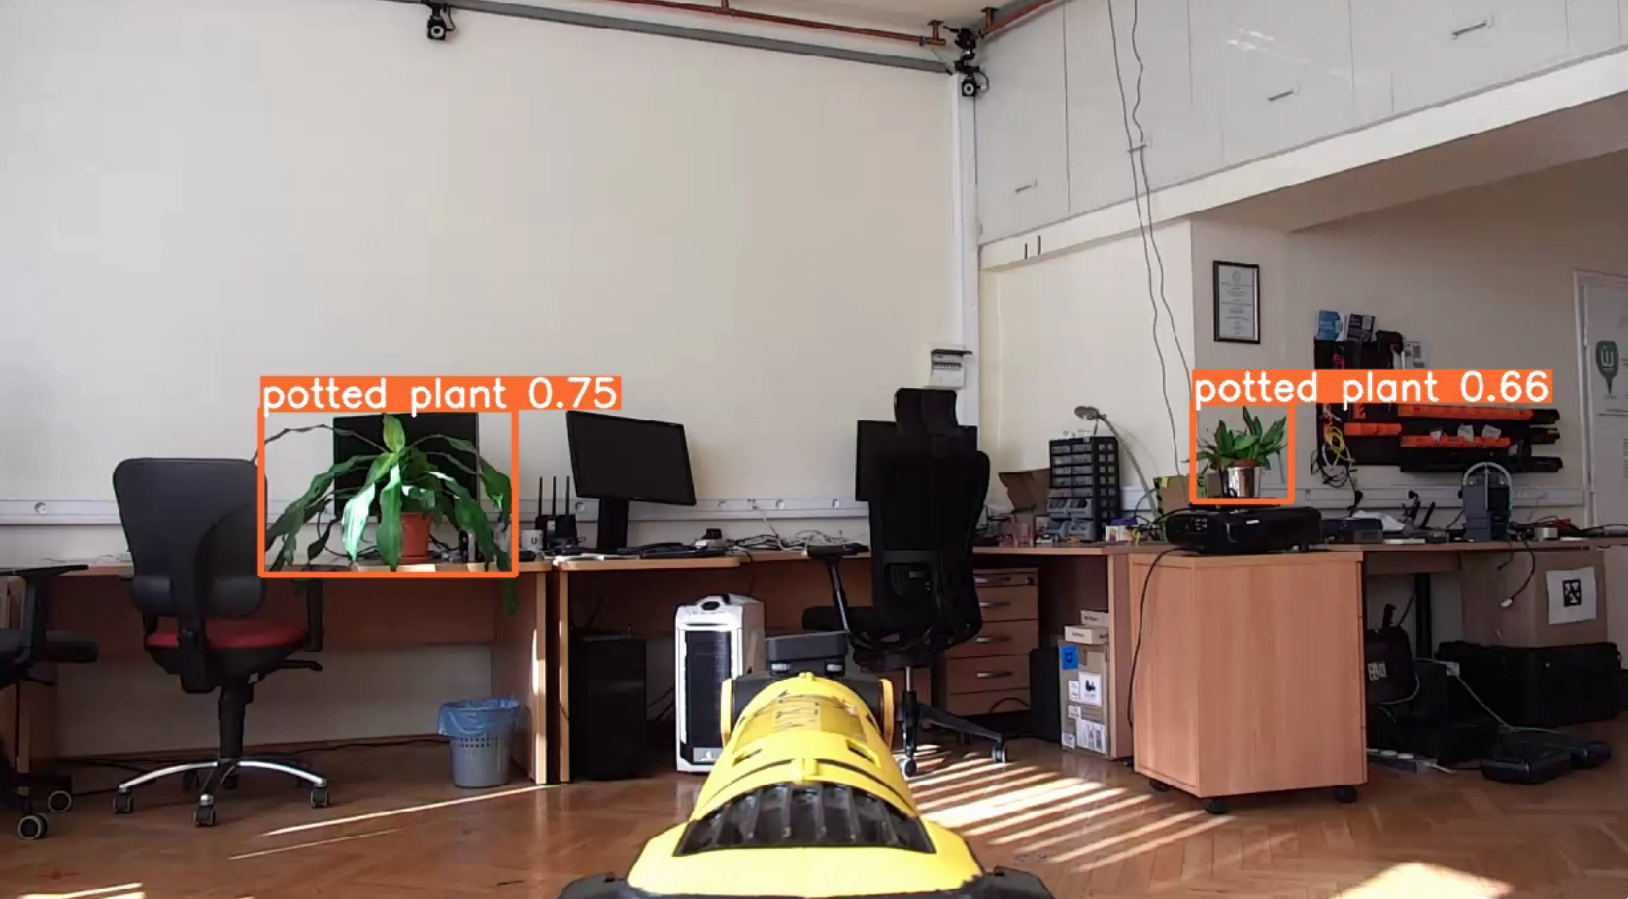
\includegraphics[width=0.95\textwidth]{assets/plant_detections.png}
	\caption{PTZ camera view of the spot robot inside of the office evaluation environment with two plants being detected.}
	\label{fig:plant_detections}
\end{figure}

\section{Simulation Setup}
To ensure the applicability of the solution on other robotic platforms and to easily test the methods in various environments without the need to deploy a physical robot, Gazebo\footnote{Ignition Gazebo Fortress, version 6.16.0}~\cite{design_koenig_2004} was used to simulate an alternative environment and robot. Gazebo is a general-purpose simulator for robotics applications that is highly customizable via plugins and widely adapted throughout the academic community and industry.

\subsection{The Simulated Robot}
The simulated robot was designed to mirror the sensory capabilities of the Spot while still being a fundamentally different platform to demonstrate the adaptability of the implementation. The biggest difference is that it uses a wheeled differential drive base instead of a legged one. It features four body-mounted surround stereo cameras for depth sensing and a fully functional simulated PTZ camera on top.

\begin{figure}[h]
	\centering
	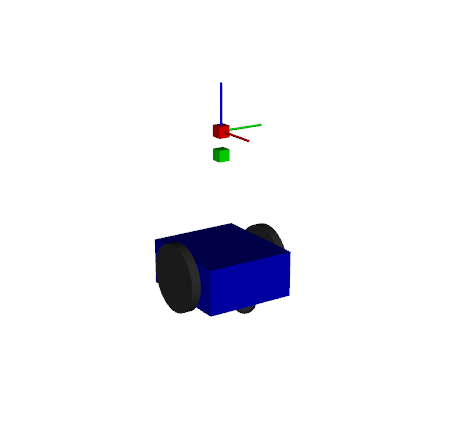
\includegraphics[width=0.6\textwidth]{assets/robot.png}
	\caption{Image of the simulated robot. It consists of a blue rectangular base with two differential drive wheels as well as a PTZ camera (red cube) and four surround stereo cameras (green cube).}
	\label{fig:simbot}
\end{figure}

While Gazebo natively supports depth and RGB cameras, emulating the Pan, Tilt, and Zoom capabilities required a custom approach. Panning and tilting is achieved by mounting the camera on two invisible revolute links controlled via joint effort controllers. For zooming, the most reliable approach we found in Gazebo was to give the camera sensor a very high base resolution. The system then computes the zoom by cropping the respective image patch based on the desired field of view and resizing it to the nominal resolution before publishing. Robot state and sensor outputs, including image streams and commands for base and PTZ camera control are mapped to ROS~2 topics. Figure~\ref{fig:simbot} shows the simplistic robot.

\subsection{Simulation Environment}
As an alternative to the office environment, we chose a common scenario within robotic applications: an indoor warehouse. More specifically, the OpenRobotics\footnote{\url{https://www.openrobotics.org/}} Depot environment~\cite{GazeboFuel-OpenRobotics-Depot}. Several objects were scattered throughout the environment. In the final setup, we decided that the robot should look for suitcases and placed six of them in the environment for the robot to find. This was a fitting decision because suitcases are a class within the COCO dataset, models are freely available from OpenRobotics as well, and a suitcase is a good demonstration of an object that reports a higher confidence score as the robot zooms in on it. Figure~\ref{fig:depot} shows the simulation environment used for the evaluation experiments.

\begin{figure}[h]
	\centering
	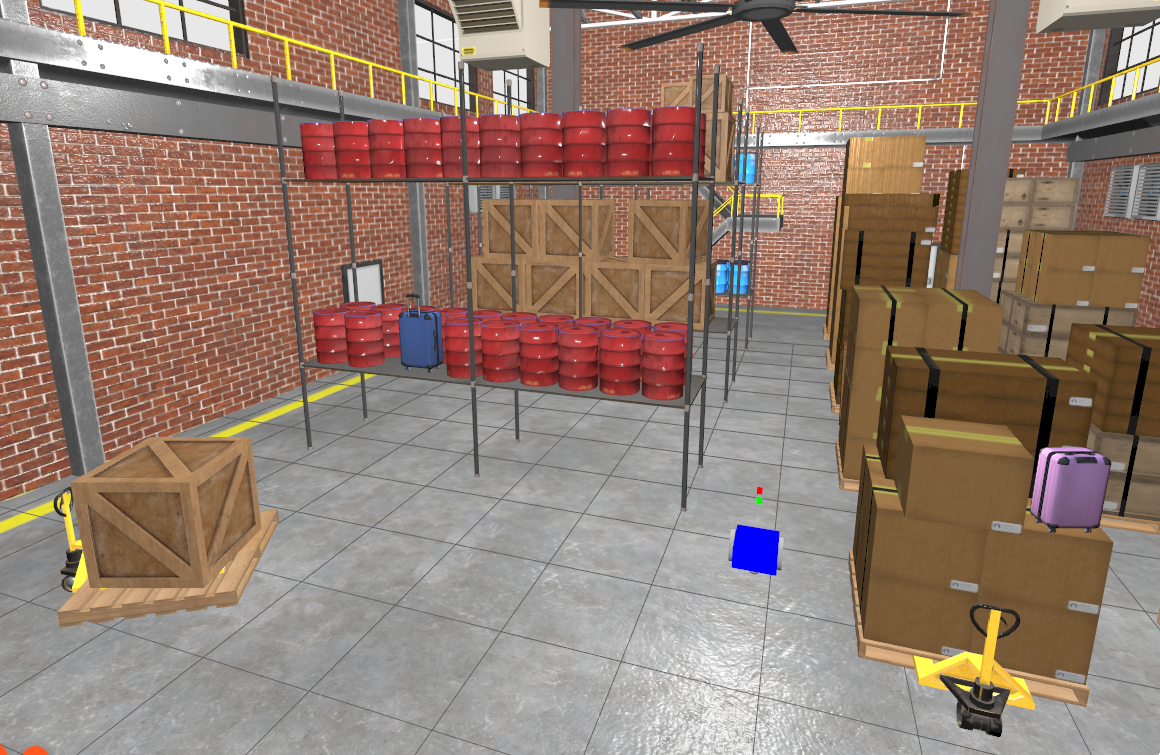
\includegraphics[width=0.8\textwidth]{assets/depot_w_robot.png}
	\caption{An example of the simulation in Gazebo with the robot inside the depot environment. Two suitcases that have been placed as target objects can be seen.}
	\label{fig:depot}
\end{figure}

\section{Experiment Setup}
Both the real-world and the simulation experiments share the same task definition, procedure and stopping criteria. The only difference is the environment and the number and class of objects to look for (plants in the real environment, suitcases in simulation).

\subsection{Task Definition}
The task to perform is the following: Within an enclosed environment, the robot should actively explore until a predefined number of target objects is found or there are no new frontiers available, meaning that the accessible geometric volume is fully explored. As part of the stopping criteria, when all target objects are found, the system keeps running for an additional 60 seconds. This allows for the initial estimate of the last objects' detection to settle to something more stable. Defining the stopping criteria in this way lets us compare the efficiency of different search strategies directly by the number of objects found and the time needed to do so.

All experiments where conducted placing the robot at the same starting position. For the real world experiments we put careful attention as well to keep other factors like the lighting and the battery charge level as similar as possible.

\subsection{Exploration Strategies}
In order to evaluate the impact of active search using a PTZ camera, we compare the following three strategies:

\begin{description}
    \item[Passive Search:] This strategy acts as a baseline to compare the other two strategies against. It keeps the PTZ camera gaze constantly straight ahead and explores the environment solely based on the geometric frontier information received from the 3D depth information.

    \item[Active Search:] Additionally to the frontier-based geometric exploration of the passive search, this strategy performs a 360-degree sweep scan with the PTZ camera whenever a frontier is reached in order to spot more objects and gain multiple viewing angles on them.

    \item[Active Search with Confirmation:] This strategy performs the same scan as the active search. Additionally, after scanning the environment, all current object hypotheses with a detection confidence get dynamically inspected with an adequate zoom level to confirm the objects in high resolution.
\end{description}

\subsection{Evaluation Metrics}
To compare the different strategies presented above, our analysis pipeline collects logging variables for each run. The following metrics are aggregated for comparison:

\begin{description}
    \item[Time passed:] The duration in seconds since the search sequence started.
    \item[Base Movement:] Cumulative translation of the robot's footprint frame through the environment in meters.
    \item[Energy Used (Spot Only):] On the physical Spot platform, we record the battery percentage drained over the course of the experiment.
    \item[Number of Objects:] The number of objects detected and successfully associated and tracker in the map.
    \item[Average Confidence] The average reported YOLO detection confidence aggregated across all tracked target objects. For each object we remember the highest detection associated with that object and average this metric across all objects found.
    \item[Average Geometric Certainty] The average trace of the 3D marginal covariance matrices representing the probabilistic certainty of all object estimates in the factor graph. If this metric is high it mean that the system is uncertain about the geometric estimates. The more different views of an object it aggregates, the smaller the trace of the covariance will become.
    \item[Average Geometric Error (Simulation Only):] The absolute euclidean distance error for object coordinate estimations compared directly against the ground truth Gazebo poses.
\end{description}

Chapter~\ref{ch:results} will present and discuss these metrics across several experiments both in simulation as well as in the real world. Finally, Chapter~\ref{ch:conclusion} concludes this thesis with a summary of findings and contributions as well as an outlook on future work.

\chapter{Results and Discussion}
\label{ch:results}
In this chapter, we present and analyze the results of the experiments described previously. Several plots detailing various exploration and object search metrics are examined. We also briefly compare the simulation results with those obtained in the real-world scenario.

\section{Simulation Experiments}

\begin{figure}[h]
    \centering

    \makebox[\textwidth][c]{
        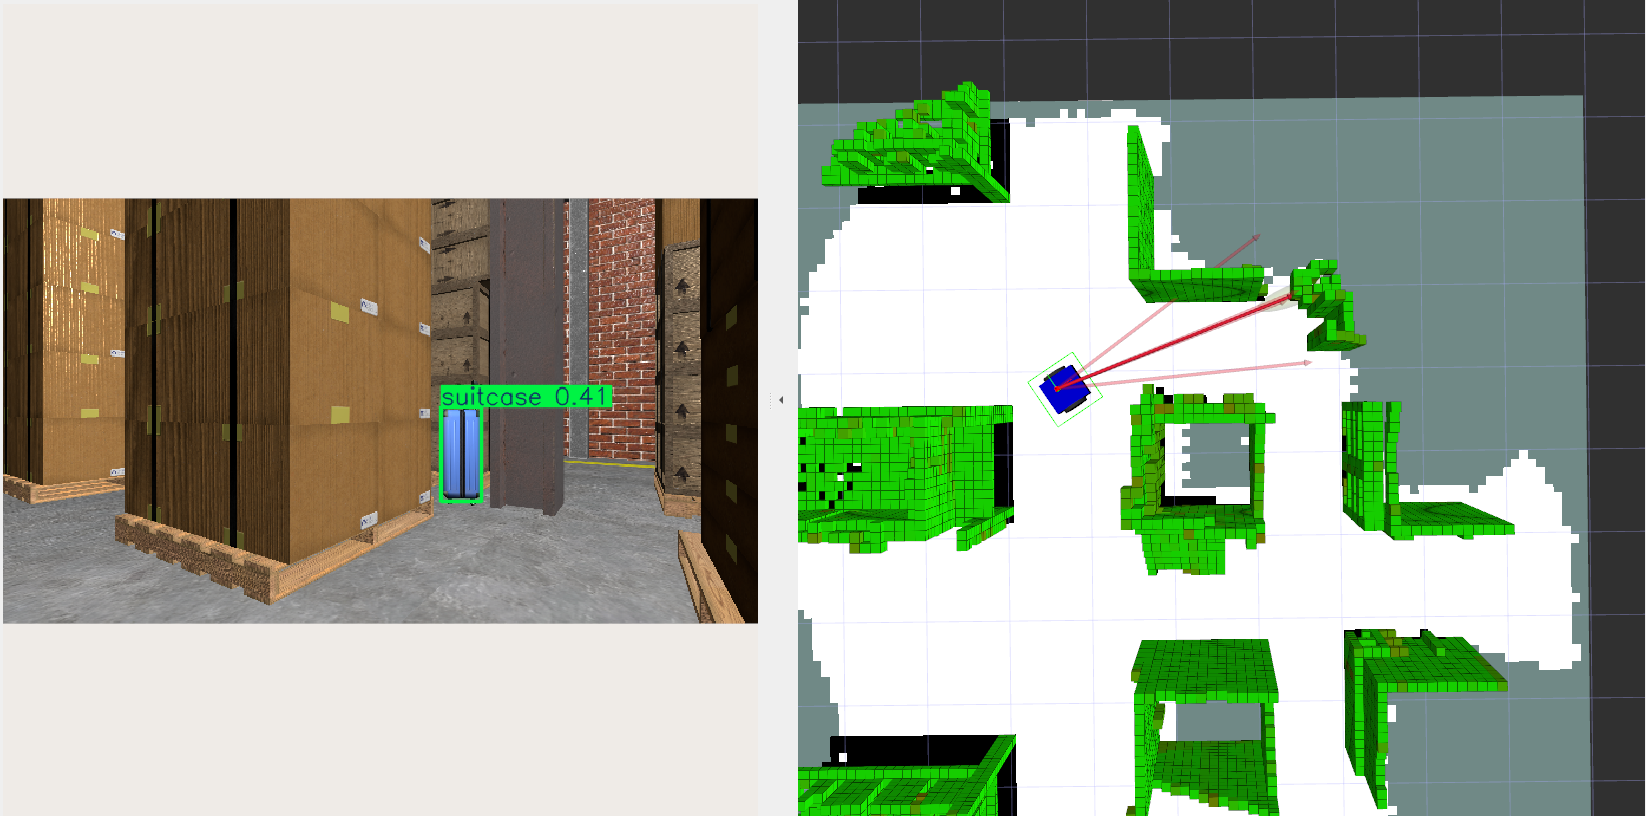
\includegraphics[width=1.2\textwidth]{assets/result_sim_in_action.png}
    }
    \caption{PTZ camera view of the depot environment during an simulation experiment run (left) and the RViz visualization of the environment explored so far (right).}
    \label{fig:res_sim_action}
\end{figure}

The simulation environment was used to test the reproducibility and reliability of our solution. The final experiment was repeated 15 times in total, consisting of 5 runs for each of the three exploration strategies. The averages for each of the metrics are presented below to highlight the differences between passive and active search strategies.

Qualitatively, the system performs well in the simulated environment. Figure~\ref{fig:res_sim_action} shows that the occupancy map is built cleanly and accurately. The software pipeline runs smoothly without computational bottlenecks. Under these almost noiseless ideal conditions, the system consistently retrieves highly precise measurements, resulting in stable and reliable 3D position estimates for the discovered objects.

\begin{figure}[h]
	\centering
	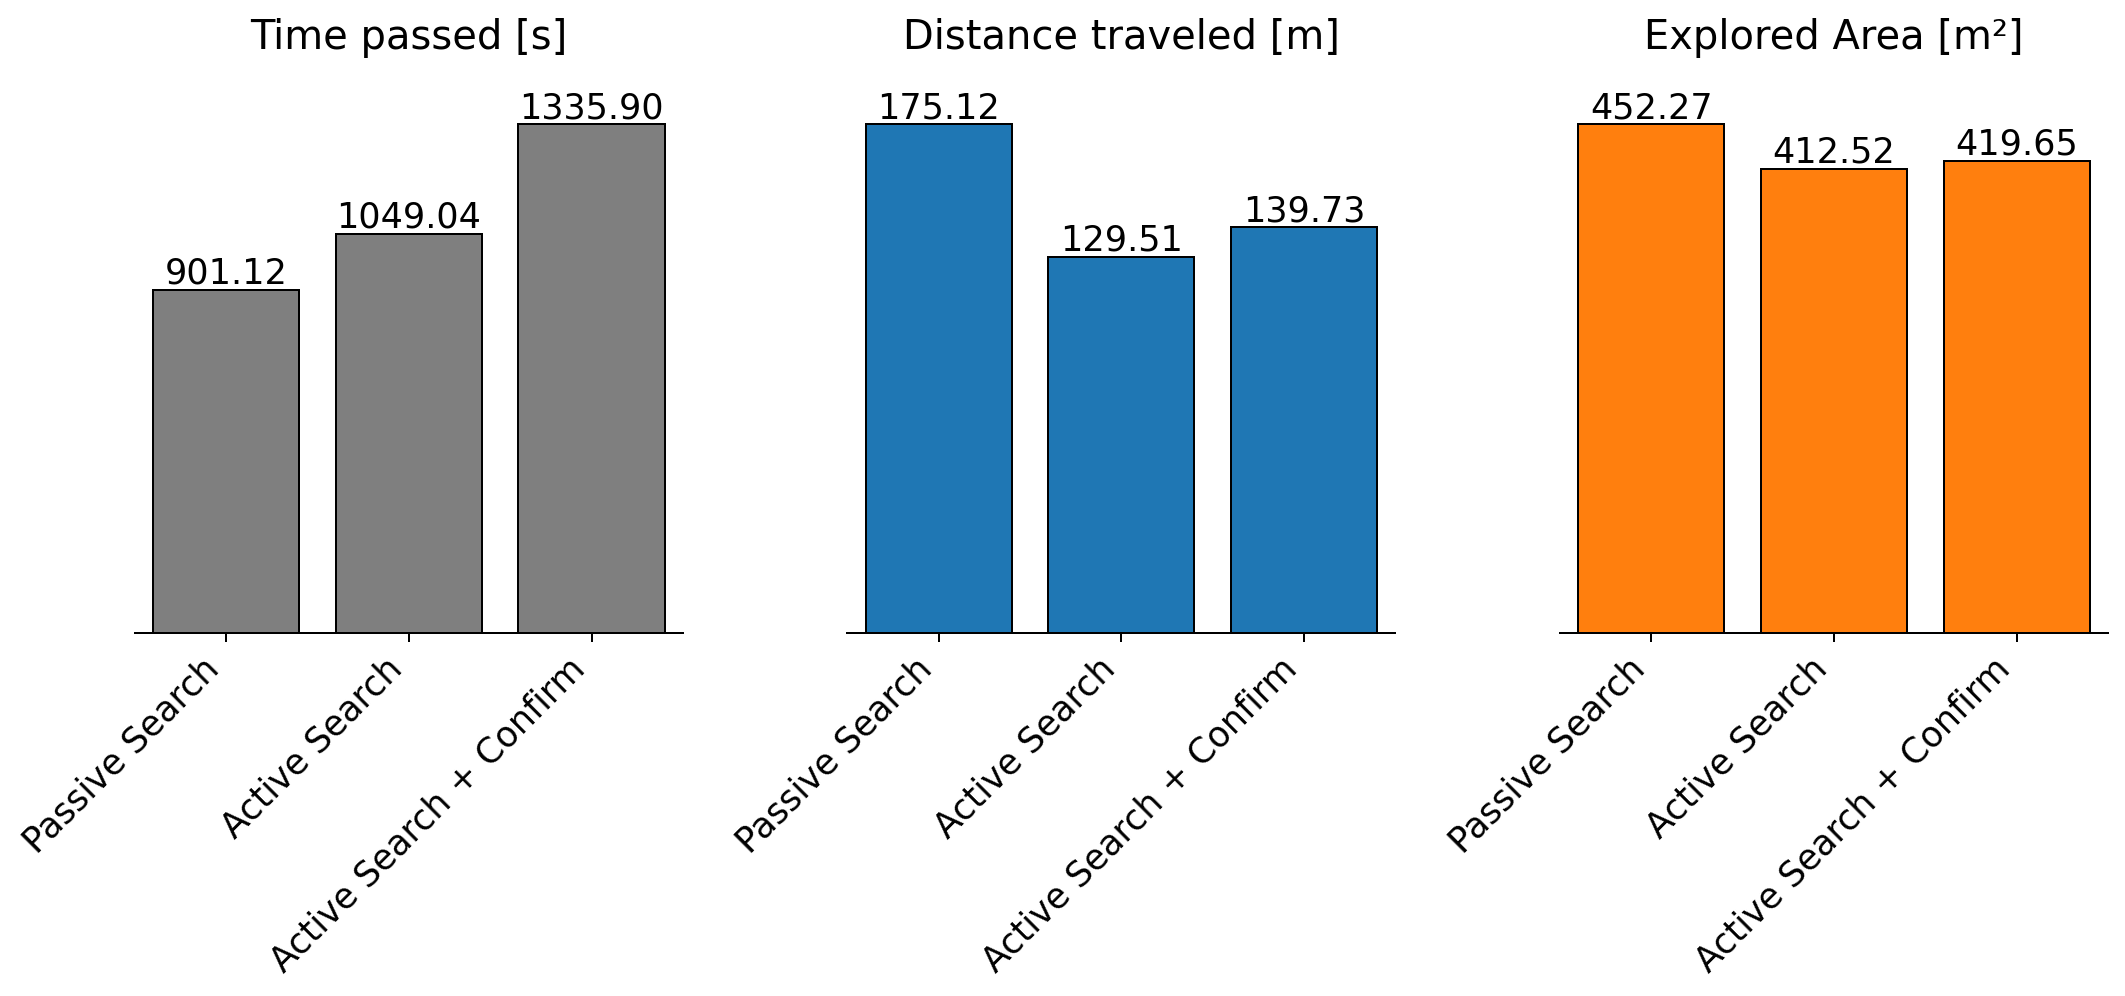
\includegraphics[width=0.9\textwidth]{assets/results_sim_bar_01.png}
	\caption{Final average values for the runtime, distance traveled, and area explored metrics for five simulation runs of each exploration strategy.}
	\label{fig:res_sim_bar_1}
\end{figure}

Figure~\ref{fig:res_sim_bar_1} shows the average runtime, distance traveled, and area explored for each exploration strategy. We can observe that the passive search is the fastest. This is because the active strategies introduce additional steps to the search, scanning and confirming landmarks at every frontier.
The passive search is also the strategy where the robot travels the most distance and uncovers the greatest area compared to the active gaze strategies. This behavior occurs because the passive strategy eventually terminates because no additional frontiers can be found, whereas the active strategies typically terminate earlier once all target objects have been identified.

\begin{figure}[h]
	\centering
	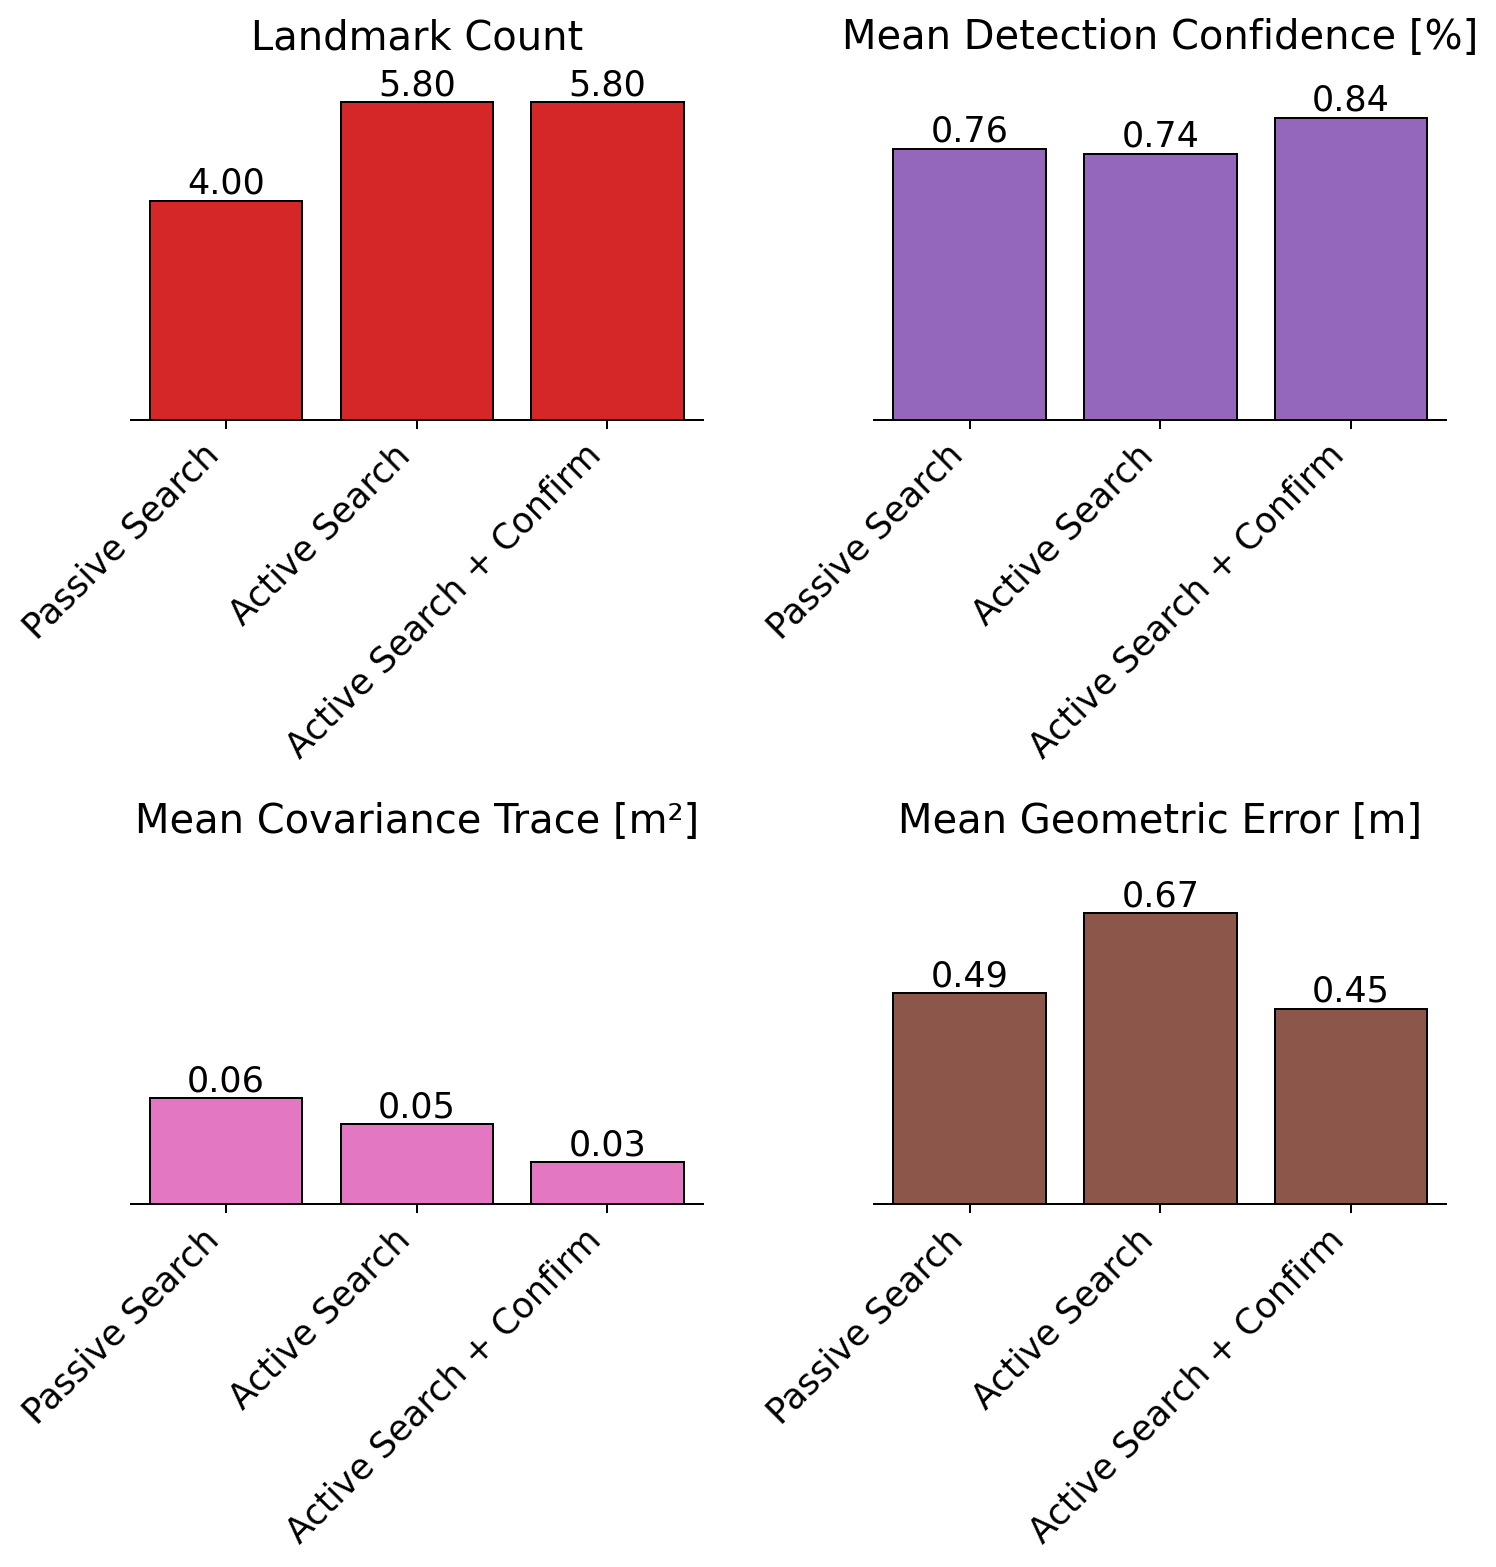
\includegraphics[width=0.65\textwidth]{assets/results_sim_bar_02.png}
	\caption{Final average values for the landmark count, mean detection confidence, mean covariance trace, and mean geometric error metrics for five simulation runs of each exploration strategy.}
	\label{fig:res_sim_bar_2}
\end{figure}

Looking at Figure~\ref{fig:res_sim_bar_2}, we can see the averages of the metrics related to object search. The most prominent difference is that the passive search, on average, only locates four out of the six objects in the environment. While this number depends heavily on the environment layout and object placement, it demonstrates that passive search strategies can miss several objects that a proper PTZ gaze control can find. 

When assessing the results for covariance trace and geometric error, we observe that the active search with confirmation performs better than the active search without confirmation. Intuitively, this can be explained by the fact that the additional viewpoints obtained during confirmation steps at every frontier lead to a better and more certain geometric estimate of the objects' positions. Similarly, the higher detection confidence is a result of the additional zoom-in on the target object, which provides a higher resolution and more detailed image for the YOLO detection model.

Unexpectedly, however, we notice that the mean geometric error appears better for the passive strategy than for the simple active search without confirmation. Upon investigating this outcome, we found that it is mostly due to a selection bias: the objects missed by the passive search are generally more difficult to find and can only be spotted from a limited number of viewpoints. Thus, without an object confirmation step, these "tricky" objects are harder to accurately estimate, negatively impacting the average error of the active method that successfully locates them without afterwards confirming them.

Figure~\ref{fig:res_sim_chart} in the appendix shows a plot of all the tracked metrics over time of three selected simulation run for comparison. 

\section{Real-World Experiments}
The real-world experiments demonstrate the feasibility of our solution in a physical scenario. The results of three runs, one for each exploration strategy within the same environment, are analyzed below.

\begin{figure}[h]
    \centering

    \makebox[\textwidth][c]{
        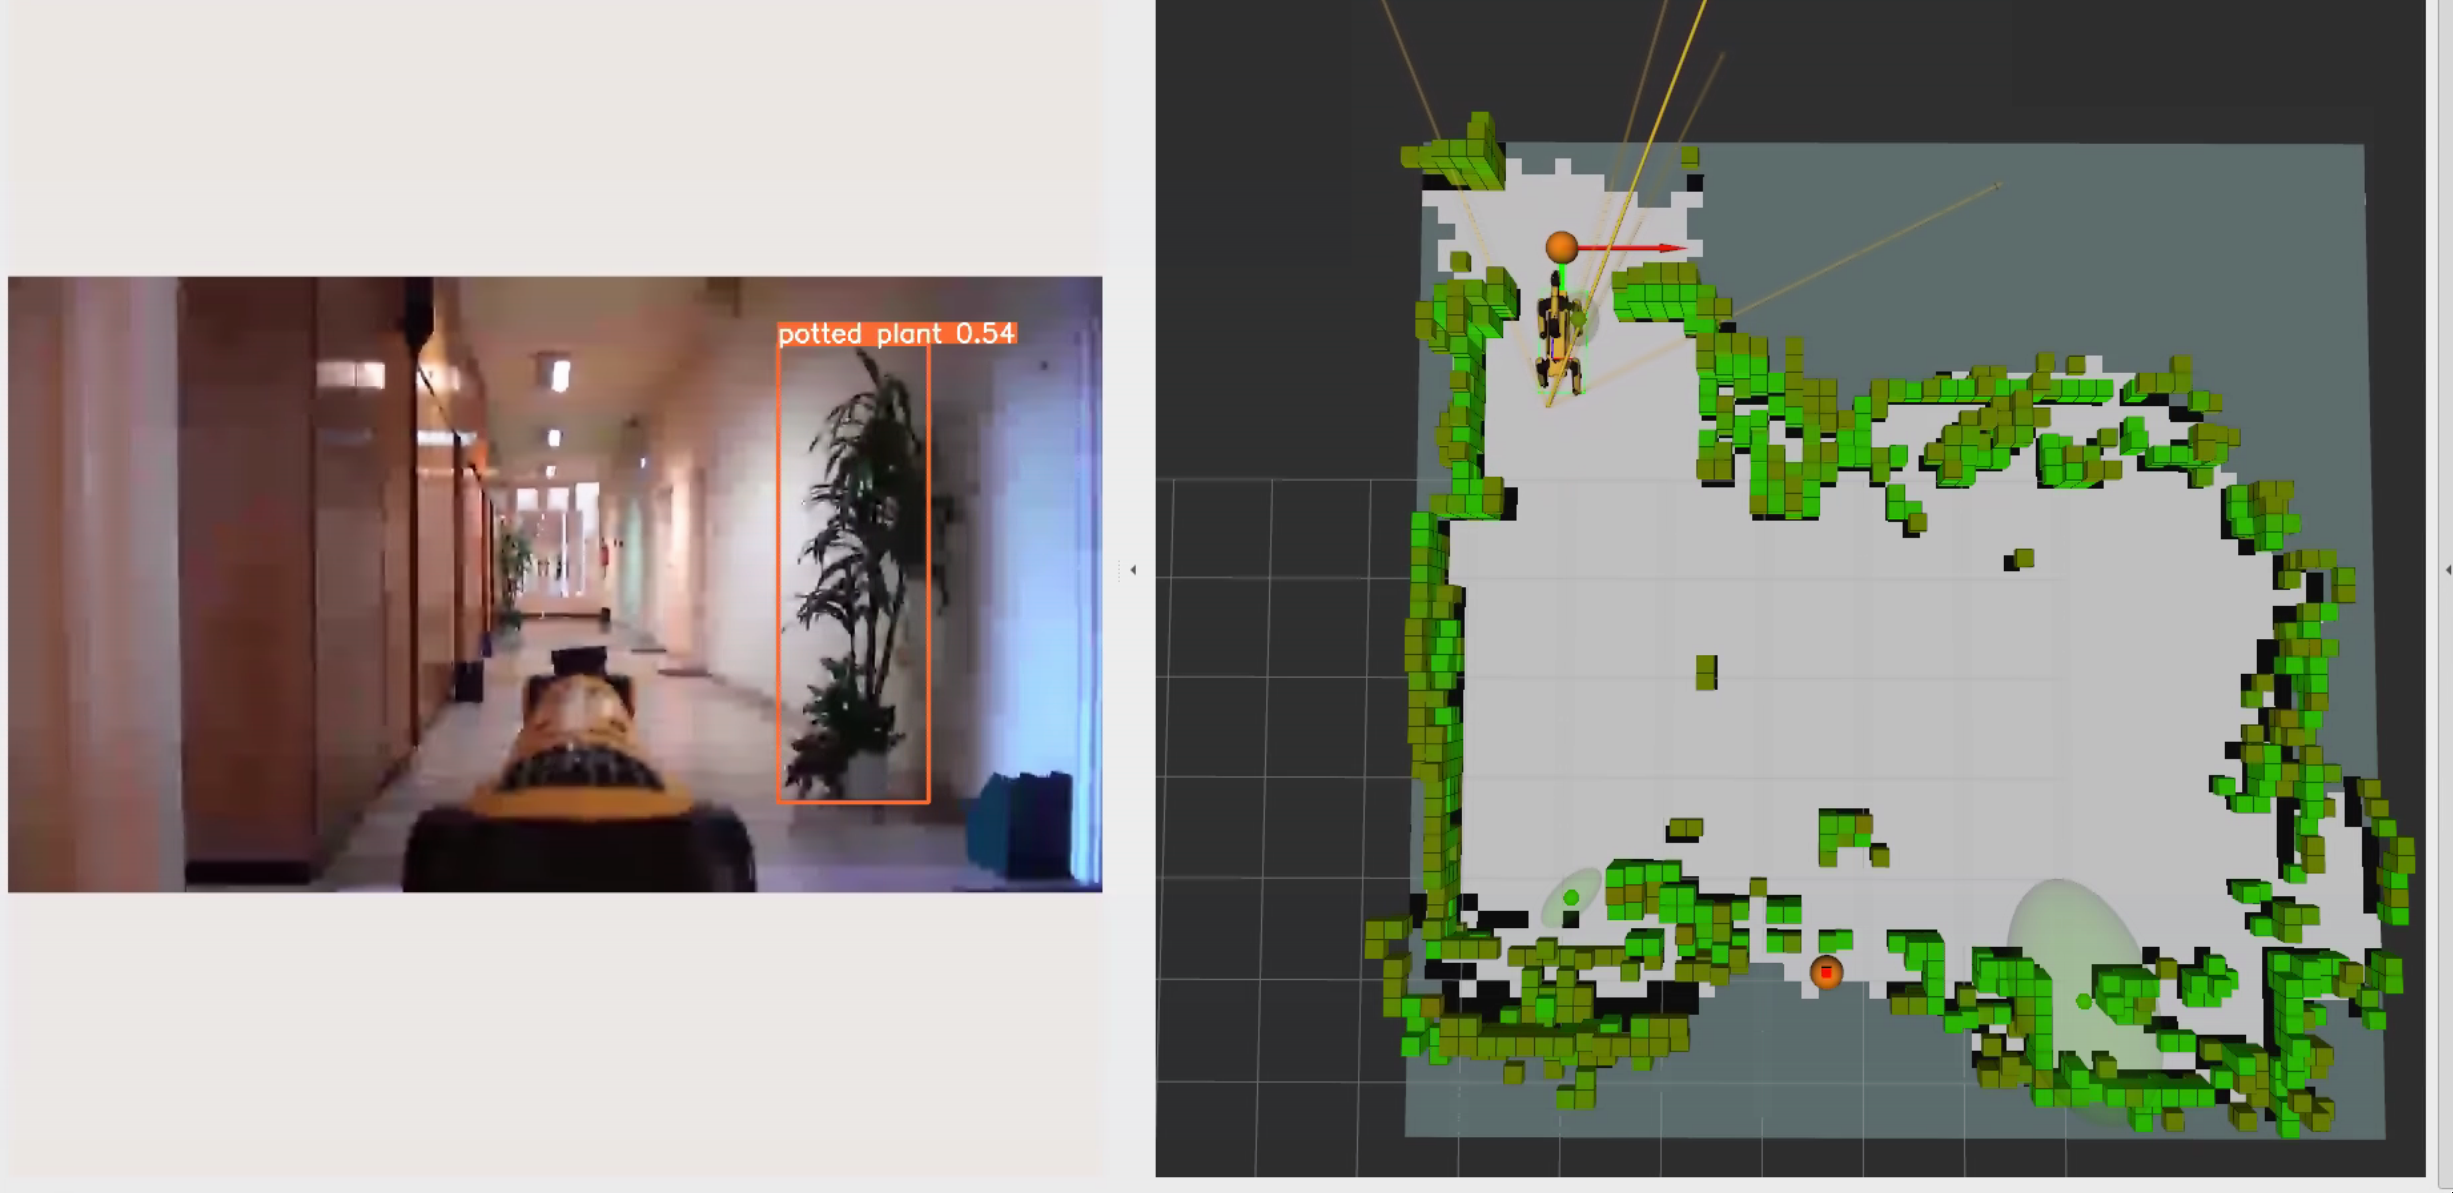
\includegraphics[width=1.2\textwidth]{assets/result_spotty_in_action.png}
    }
    \caption{PTZ camera view of a hallway during the final real-world experiment (left) and the RViz visualization of the environment explored so far (right).}
    \label{fig:res_action}
\end{figure}

In Figure~\ref{fig:res_action}, we can see the robot exploring its environment as visualized in RViz. As expected, the generated map is slightly noisier than in the simulation, but the target plants are still being detected and localized successfully. What is not apparent from the figure is that the real-world execution is notably slower than the simulation. This drop in speed is primarily due to computational limitations on the portable computer and communication bottlenecks with the robot interfaces.

\begin{figure}[h]
	\centering
	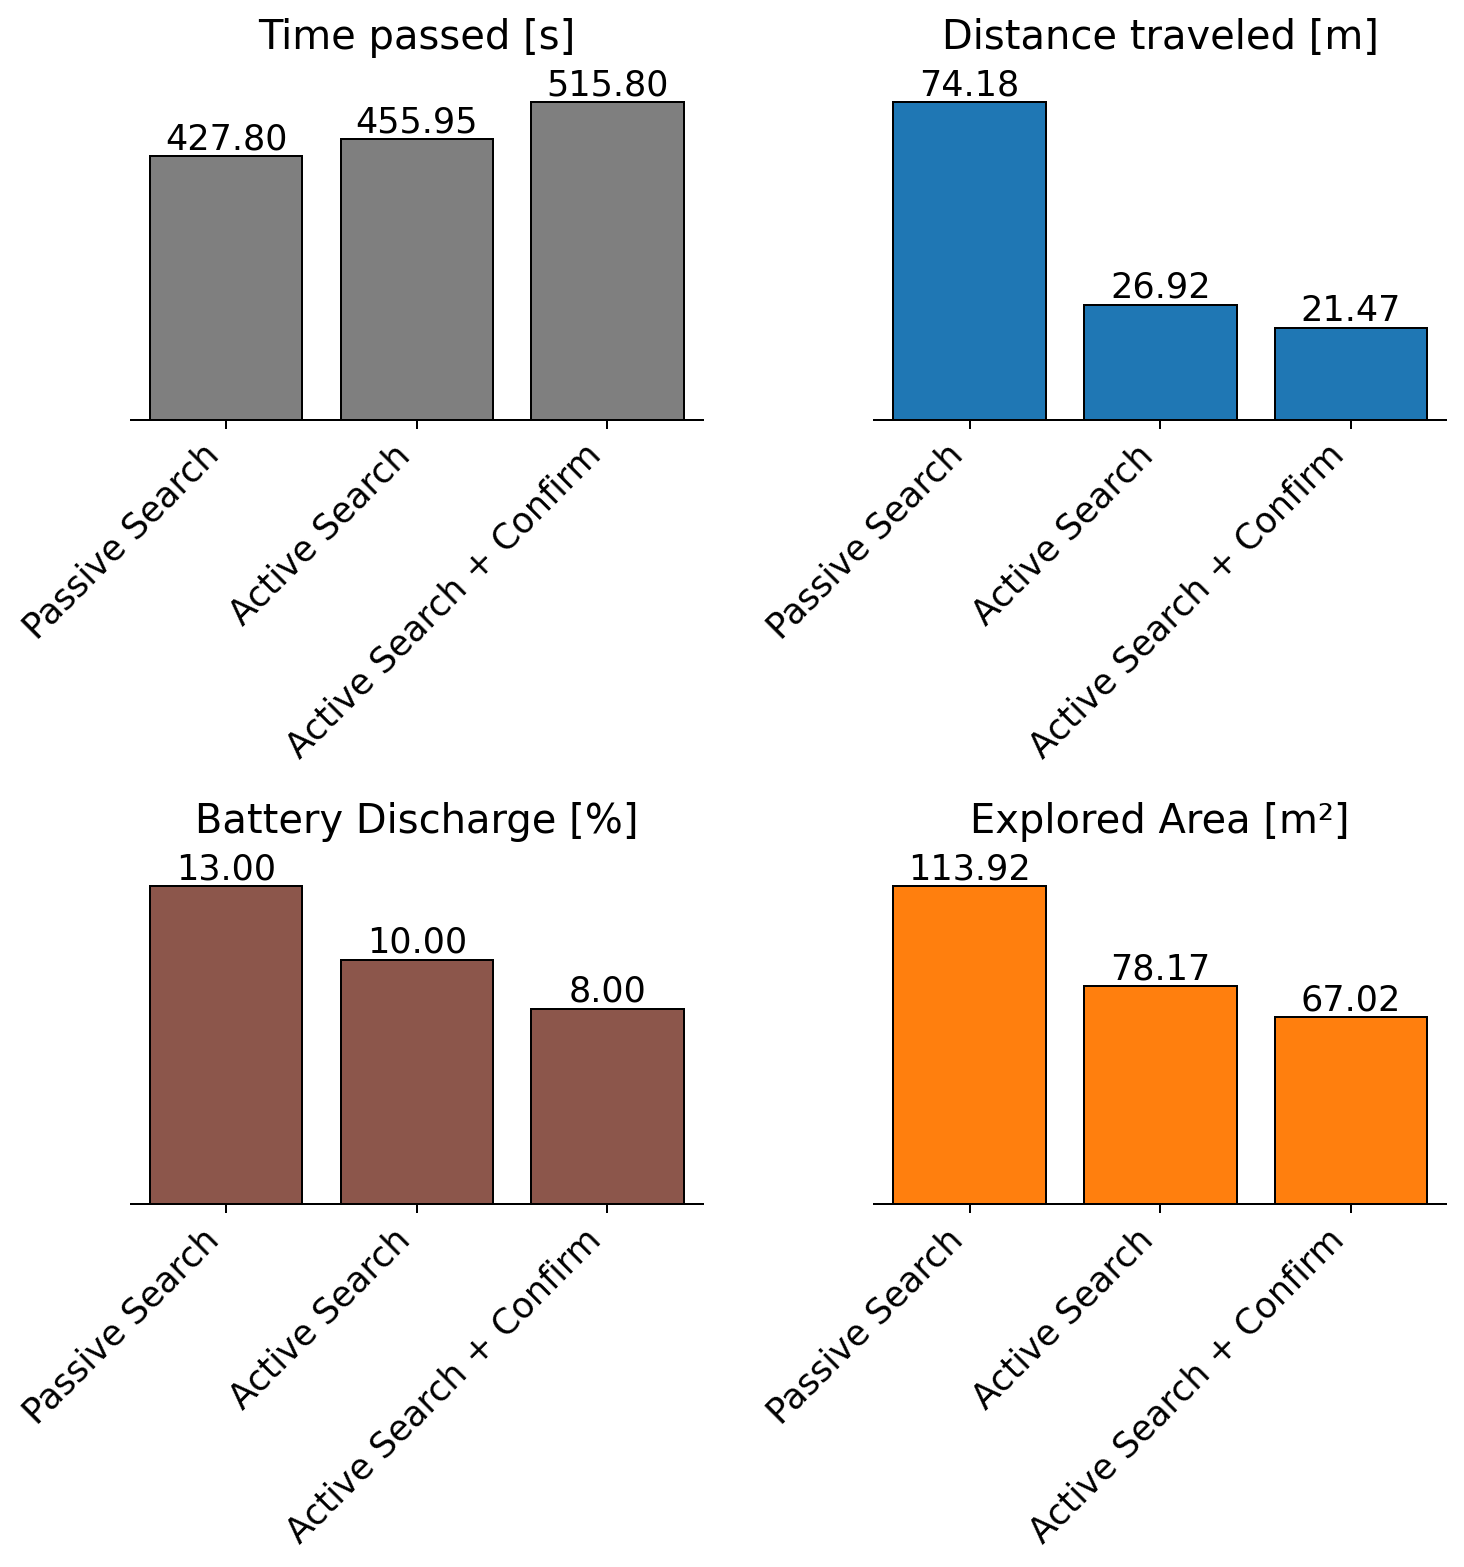
\includegraphics[width=0.65\textwidth]{assets/results_spot_bar_01.png}
	\caption{Final values for the runtime, distance traveled, and area explored metrics across three real-world runs, one for each exploration strategy.}
	\label{fig:res_spot_bar_1}
\end{figure}

In Figure~\ref{fig:res_spot_bar_1}, we see trends similar to the simulation results: the passive strategy is the fastest, explores the most area, and requires the robot to move the most. Because we tracked the battery discharge during the real-world exploration, we can examine the impact of this movement. Even though the passive search had the shortest operation time, the frequent physical movement of the robot's legs led to the highest total battery discharge. By calculating the battery discharge per minute for these runs, we observe the following values:

 \begin{itemize}
     \item \textbf{Passive Search:} 1.83 \% per minute
     \item \textbf{Active Search:} 1.31 \% per minute
     \item \textbf{Active Search + Confirmation:} 0.93 \% per minute
 \end{itemize}

While these specific numbers only reflect three runs and in practice depend on many environmental factors, such as temperature, floor conditions, and room layout, the difference remains noticeable. It illustrates that by employing a smart PTZ control strategy, unnecessary physical movement is reduced, lowering the battery discharge rate and thus extending the potential operation time of the robot in systems where battery life is critical.

\begin{figure}[h]
	\centering
	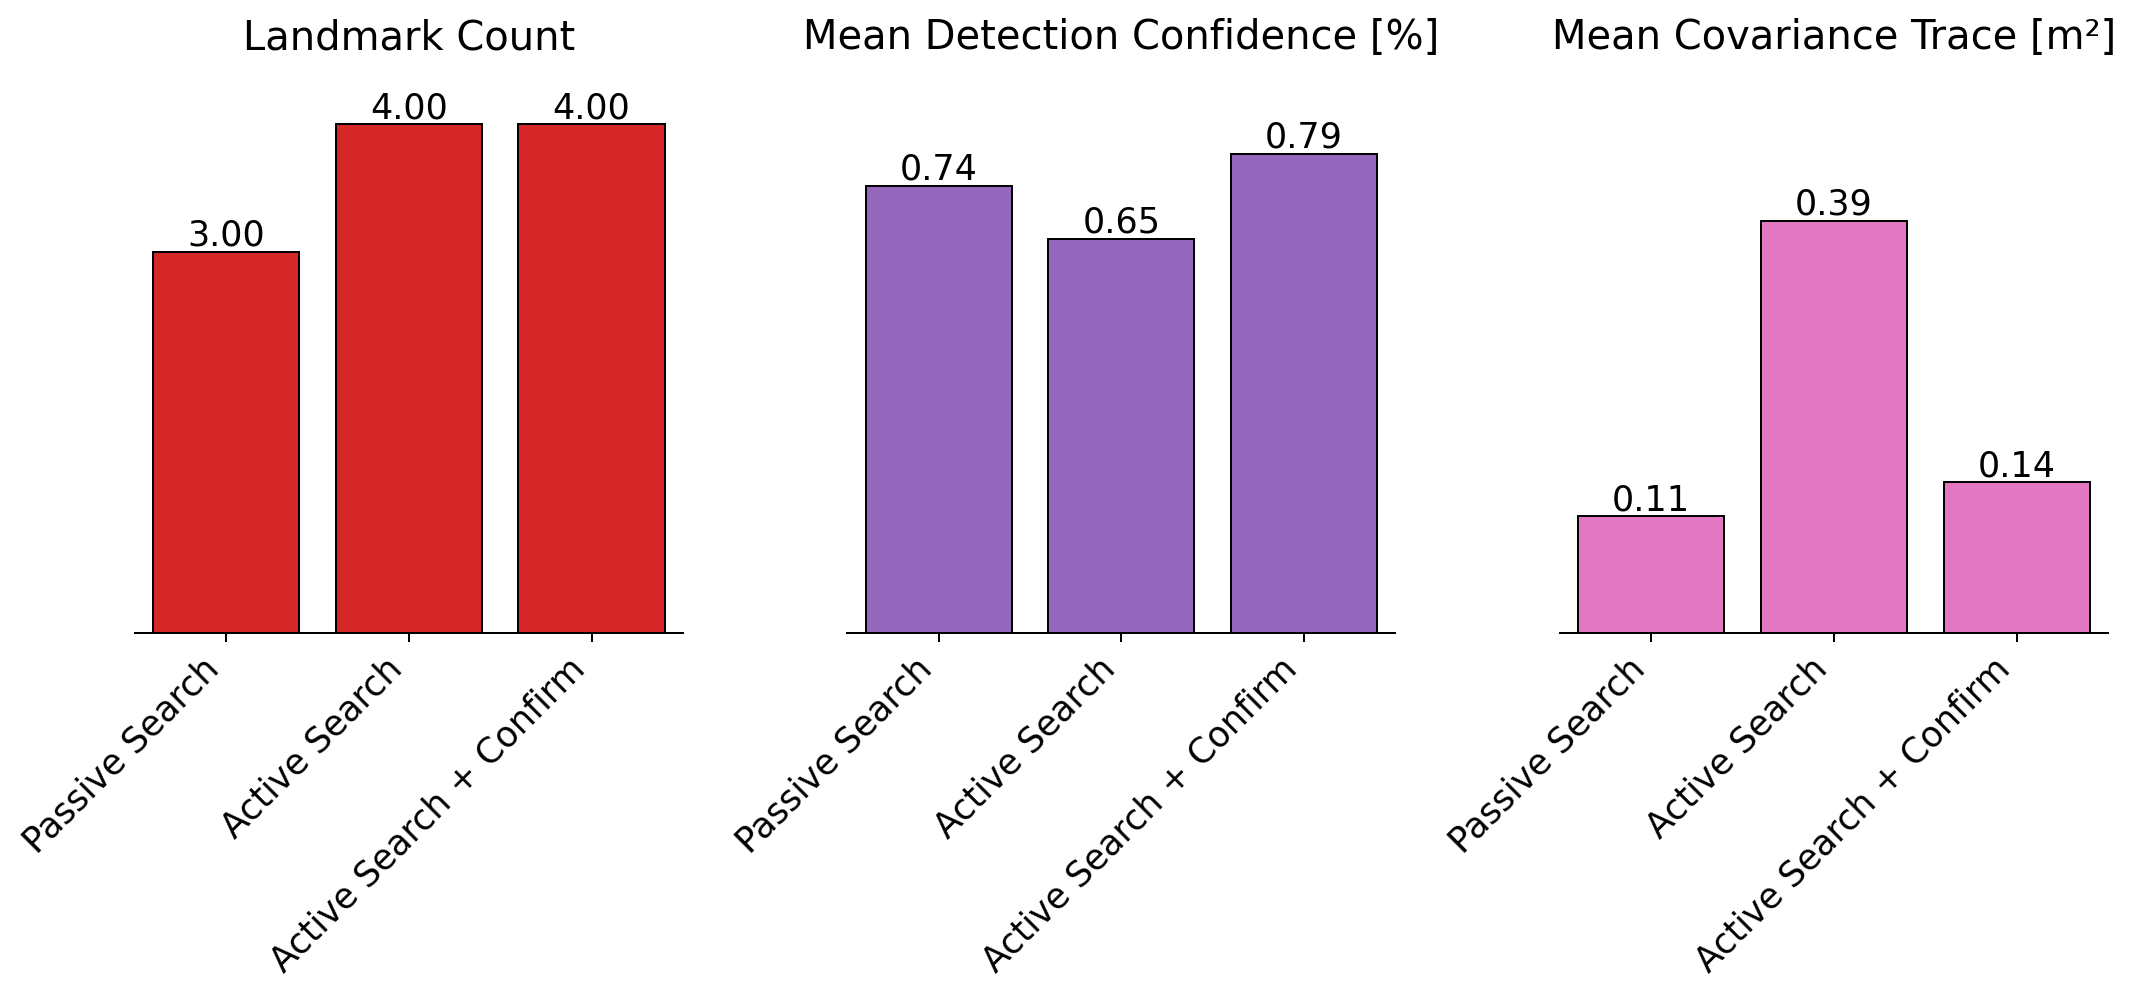
\includegraphics[width=0.9\textwidth]{assets/results_spot_bar_02.png}
	\caption{Final values for the landmark count, mean detection confidence, mean covariance trace, and mean geometric error metrics across three real-world runs, one for each exploration strategy.}
	\label{fig:res_spot_bar_2}
\end{figure}

Figure~\ref{fig:res_spot_bar_2} displays relationships that largely mirror the simulation results. In the passive search run, one of the target objects was missed entirely because the robot never turned in its direction, walking past it without the object ever entering the camera's field of view. Additionally, the data confirms that the extra confirmation step successfully helps narrow down the covariance of the object location estimates and increases detection confidence.

We do notice that the passive search achieved the best result for mean object location covariance alongside a solid detection confidence. While in the simulation this effect was caused by the selection bias of the passive strategy missing difficult objects, in the real-world experiment it stems from the robot's physical trajectory. In the passive search scenario the robot traveled along the entire length of the corridor twice, gaining several high-quality angles of the plants located there. The active search without confirmation, on the other hand, detected the plants situated far down the corridor quite early, triggering the stopping criteria because those where the last plants to be found. As previously described, a one-minute shutdown period occurs after all objects are found. Without an active confirmation step, this waiting time was not sufficient to capture significantly different viewpoints of the plant far back in the hallway. Consequently, the experiment concluded before the system had a chance to properly narrow down its estimate, leaving a relatively high uncertainty despite an accurate position estimate.

For the real-world experiments, obtaining precise ground-truth coordinates was impractical, so formal geometric error metrics were excluded. We did, however, review the results manually and observed that all stable center estimates fell within a radius of approximately fifty centimeters from the actual object's location, even in the worst cases.

In the appendix, Figure~\ref{fig:res_spot_chart} provides an in-detail look at how all the metrics evolved over time during the three exploration runs.

\chapter{Conclusion}
\label{ch:conclusion}

Building and testing our active visual search system gave us several clear takeaways. This chapter summarizes the findings, clarifies how they are related to the initial research questions and highlights future work possibilities.

\section{Summary of findings}
First and foremost we can see that an active search strategy bring real benefits over standard passive strategies. Depending on the mission, these benefits show up in different ways. While passive search is generally faster at simply mapping out the geometry of a room, it forces the robot to physically walk much further. Active scanning can reduce how much the robot actually has to move if the goal is to locate a number of target objects. For a legged robot like Spot, moving around takes a lot of energy. Walking less means saving battery and potentially extending the total mission time. Also, looking around actively is incredibly helpful when the robot cannot physically reach certain areas but needs to inspect them from a distance.

We also found that using the camera's optical zoom, a feature often ignored in typical exploration research, boosts search performance. By zooming in to confirm objects, the system becomes more confident in its detections because the zoomed-in images capture fine details that a wide-angle field of view misses. It also calculates more accurate 3D positions because of the combination of different view angles.

Still, the real-world setup has its limits. Our current scanning method, which pauses the robot to look around slows down the exploration process. We chose this approach because of stability issues where controlling the PTZ camera while walking resulted in a very blurry and almost unusable image stream.
Furthermore, while the onboard Jetson Orin computer has plenty of GPU power for running the YOLO detection model, the CPU and network struggle to handle the high-resolution PTZ image streams alongside the heavy 3D pointcloud data at the same time without lagging. On top of that, while the Boston Dynamics Spot is a very reliable as an industrial robot, it still lacks complete ROS integration for effortless academic research with custom or complex payloads. 

Overall, these results are very promising, especially since our search rules are relatively simple. They prove that even a basic setup combining active PTZ camera control with robot navigation can save energy and perform better than standard methods, leaving plenty of room for future improvements.

\section{Research questions revisited}

\subsection{RQ1}
\textbf{How can a robotic agent autonomously coordinate base mobility and independent camera gaze to maximize the probability of detecting a target object in an unknown environment?}

This thesis presents a complete system that showcases how several components can be  orchestrated to tackle the object search problem using a PTZ camera. The solution utilizes a standard geometric exploration module to direct the robot's base toward unexplored regions using frontier-based exploration. To maximize the probability of finding targets and ensuring reliable detections at the same time, the camera gaze is coordinated via a "stop-and-go" scanning routine. This ensures high-quality, image acquisition and visual coverage of newly accessible areas, loosely decoupling base movement from active visual inspection.

\pagebreak
\subsection{RQ2}
\textbf{How can the trade-off between sensor coverage (Field of View) and detection confidence (Resolution) be modeled?}

Visual search involves a fundamental trade-off: a wide Field of View maximizes spatial coverage but yields low-resolution images, while optical zoom provides the pixel density required for confident detection but severely restricts the sensor coverage. Our experimental results show that actively leveraging optical zoom increases overall detection confidence, proving its value. Our method decouples scanning and verifying in two steps, to balance spatial coverage and confident detections. First, the robot scans the environment at its normal zoom level to find low-confidence object hypotheses. Second, the system triggers an active confirmation phase, steering the PTZ camera and applying optical zoom to inspect these initial detections at high resolution.

\subsection{RQ3}
\textbf{How can an active visual search strategy improve search efficiency and detection range compared to standard passive exploration baselines?}

The results from both simulated and real-world experiments demonstrate that an active visual search strategy can enhance overall search efficiency for object detection tasks. While the passive exploration runs were generally faster at mapping out geometry, they force the robot to uncover more area and hence travel longer distances.  An active search strategy on the other hand allows the system to inspect its surroundings more efficiently by separating the camera gaze from the base movement,. This reduces the overall base movement necessary to locate all target objects, which in turn leads to energy savings during operation. Furthermore, integrating optical zoom to confirm object detections proved to be very valuable. Zooming extends the robust detection range by providing higher resolution images of distant objects, which enhances detection confidence and makes 3D position estimates more accurate.

\section{Contributions}

\textbf{Modular Active Search Implementation}

We developed a complete, hardware-agnostic ROS~2 software stack that integrates spatial exploration, target detection, and PTZ camera control. By keeping the core algorithms decoupled from the physical robot drivers, this framework can be easily adapted to and deployed on any mobile base utilizing the standard Nav2 stack.
    
\textbf{Custom PTZ Integration for the Spot Robot}

To bridge the gap between Boston Dynamics' proprietary software and the open-source ROS ecosystem, we implemented a custom ROS~2 package. This tool set enables the "SPOT~Cam+IR" payload to work with standard setups, providing a straightforward interface for camera streams, PTZ commands, and coordinate (TF) tree transformations.

\textbf{Simulation Environment}

For faster prototyping, reproducible testing, and future development without the need for physical hardware, we designed a comprehensive Gazebo simulation setup. This includes a differential-drive robot model equipped with an emulated PTZ camera and surround depth sensors, deployed within an indoor warehouse environment.

The complete source code including the search architecture, the custom Spot payload integration, and the simulation environment is available as an open-access repository\footnote{\url{https://master-thesis.lolo.place}}.
    
\textbf{Conceptual Proof and Experimental Benchmark}

Through real-world and simulation experiments, this work serves as a practical Proof of Concept demonstrating that actively coordinating base mobility with independent PTZ gaze control can improve search outcomes. Our comparison shows that active sensing, especially when using zoom for target confirmation, enhances object localization accuracy and detection confidence and reduces overall base movement compared to passive search strategies.

\section{Future Work}
This work can be understood as a foundation for many more sophisticated active search strategies for the Boston Dynamics Spot. Although we successfully demonstrate that PTZ cameras can be used to make the task of object search more efficient, there is still considerable room for improvement regarding PTZ control integration and overall system performance.

\begin{description}
    \item[Hardware and Interface Optimization:] The experiments on the Spot robot highlighted clear hardware limitations. While the Jetson Orin has a strong GPU unit, its CPU capabilities were not enough to smoothly process the high-resolution PTZ image stream at the same time with the dense 3D point clouds and the rest of our implementation. Future work could work on improved hardware interfaces for the Spot robot and optimize the ROS~2 wrappers to ho mitigate this.
    
    \item[Continuous Move, Gaze, and Zoom:] Without the tight hardware limitations, the "stop-and-go" scanning pipeline can easily be improved upon. Future implementations should focus on active scanning that manipulates the mechanical PTZ camera while the robot is in motion. The system could formulate an optimization problem that balances base movement, camera gaze and optical zoom in real time.
    
    \item[Semantic and Attention-based Search:] Currently, our active search scans the environment with a uniform 360-degree sweep. Future implementations could use spatial semantics to direct the camera's gaze intelligently. By incorporating semantic mapping structures, similar to recent advancements utilizing semantic maps \cite{semantic_asgharivaskasi_2023, active_zhang_2024}, the system could look towards unexplored high-probability regions (e.g., scanning desks rather than the floor for a coffee cup) instead of relying on exhaustive sweeping.

\end{description}

\cleardoublepage

% Bibliography
\phantomsection
\addcontentsline{toc}{chapter}{\biblabel}
\printbibliography[title=\biblabel]
\cleardoublepage

% Appendices (optional) - useful for detailed information in long tables, many and/or large figures, etc.
\appendix
\phantomsection
\addcontentsline{toc}{chapter}{\annexlabel}

% --- Start of spacing override ---
\makeatletter
\renewcommand{\@makechapterhead}[1]{%
  \vspace*{0\p@}% <--- Kills the massive 50pt gap at the very top
  {\parindent \z@ \raggedright \normalfont
    \ifnum \c@secnumdepth >\m@ne
        \huge\bfseries \@chapapp\space \thechapter
        \par\nobreak
        \vskip 0\p@ % <--- Shrinks the gap between "Appendix X" and the title
    \fi
    \interlinepenalty\@M
    \Huge \bfseries #1\par\nobreak
    \vskip 0\p@ % <--- Shrinks the gap between the title and your first paragraph
  }}
\makeatother
% --- End of spacing override ---

\chapter{AI Usage Notice}
\label{app:ai-usage}

A number of different generative Artificial Intelligence (AI) tools were used for researching, writing and developing this thesis.

First and foremost Google Gemini\footnote{\url{https://gemini.google.com/}} was used throughout the whole process for brainstorming, concept clarification, web research and validation. This tool was also directly prompted to draft paragraphs from internal notes, code and results, refine spelling and rephrase text for the thesis report.
For the literature review, ResearchRabbit\footnote{\url{https://www.researchrabbit.ai/}} was used to organize references and find related literature and Google NotebookLM\footnote{\url{https://notebooklm.google.com/}} to assist in summarizing and relating cited academic papers.
For software implementation GitHub Copilot\footnote{\url{https://github.com/features/copilot}} was used for both inline code completions as well as complex refactoring tasks and documentation of the software.

These tools were used as a support and not to replace the core intellectual problem-solving. Prompts were always phrased as assistive requests (e.g.: "Proofread this paragraph", "Refactor this file to expose all marked variables as configuration parameters" or "Rephrase this section to make it suitable for an academic thesis") and never as to outsource the actual research or implementation process (e.g.: "Write a section about what can be concluded from the results", "Implement an algorithm to estimate and track 3D coordinates from 2D object detections")

All AI-generated outputs were evaluated and verified before being included in the final text and implementation. As the author, I take full responsibility for the correctness and completeness of all content presented in this work.

\chapter{In-depth Results}
\label{app:in-depth-results}
 \begin{figure}[h]

    \centering

    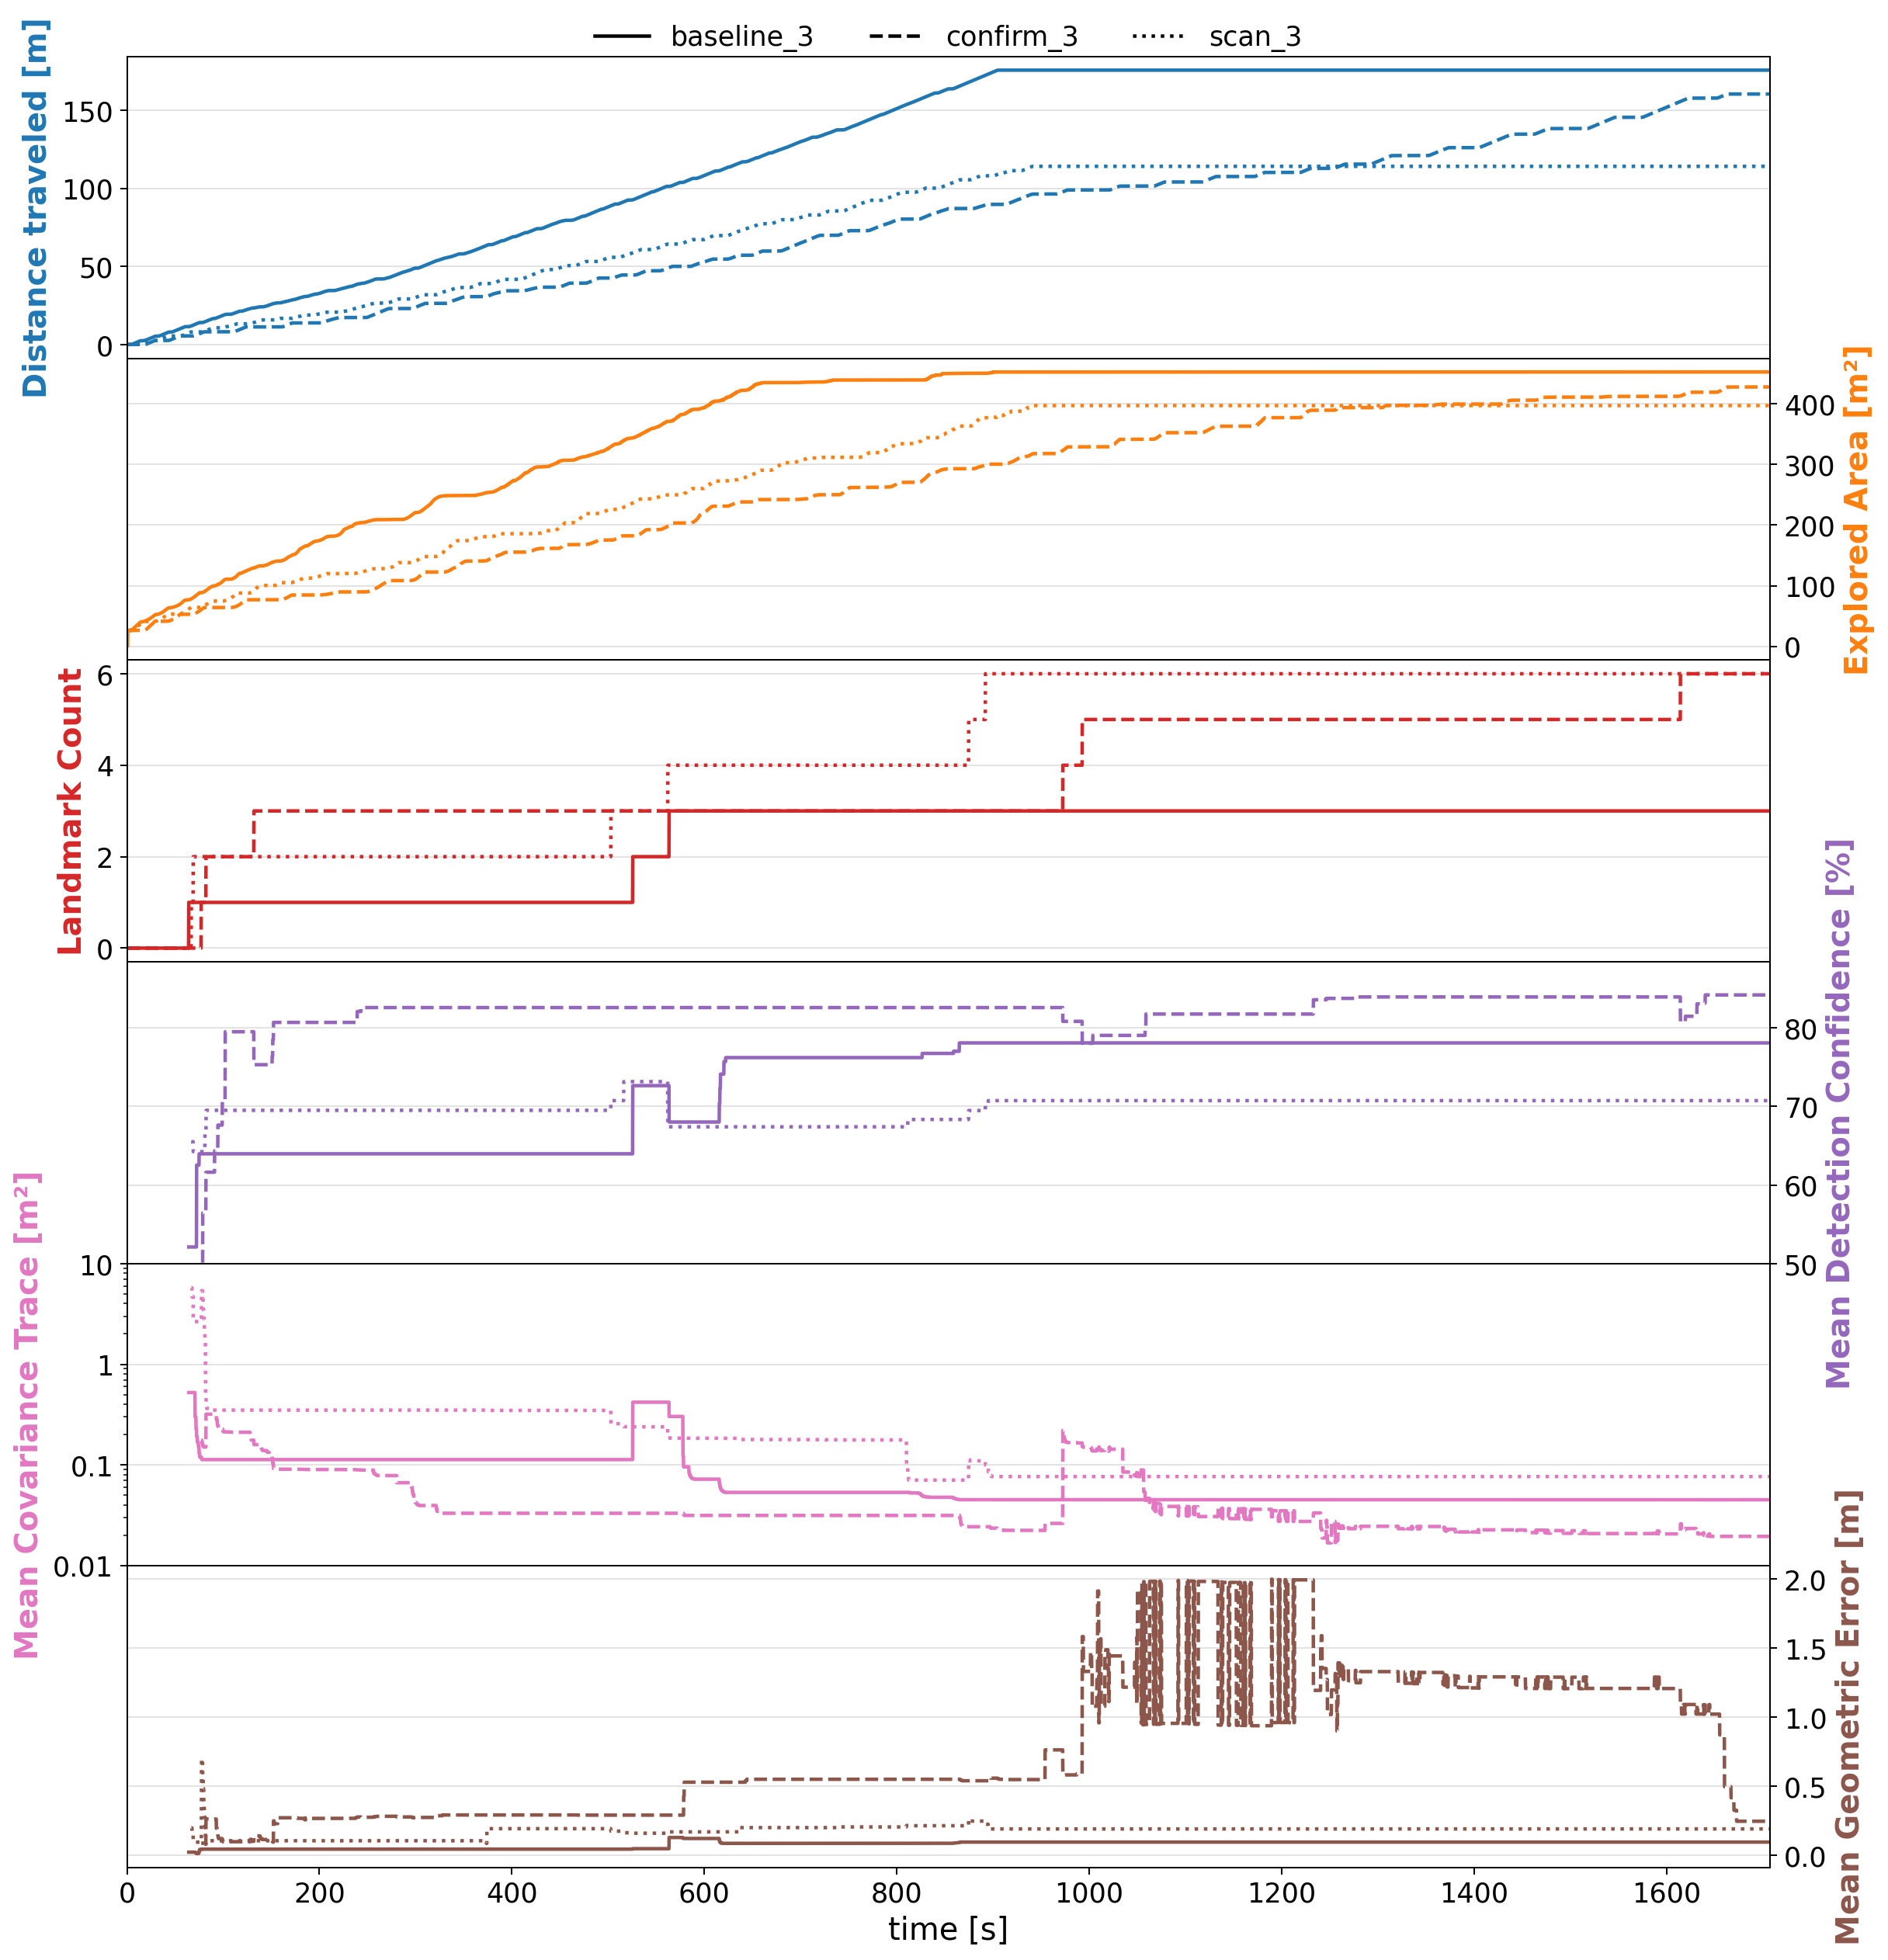
\includegraphics[width=0.95\textwidth]{assets/results_sim_chart.png}

    \caption{Comprehensive timeline of evaluation metrics during three representative simulation runs within the Gazebo depot environment. The stacked subplots track distance traveled, explored area, cumulative landmark count, mean detection confidence, mean covariance trace (logarithmic scale), and mean geometric error over the duration of the experiment. The line styles distinguish the three evaluated methodologies: Passive Search (solid line), Active Search (dotted line), and Active Search with Confirmation (dashed line).}

    \label{fig:res_sim_chart}

\end{figure}


\begin{figure}[h]

    \centering

    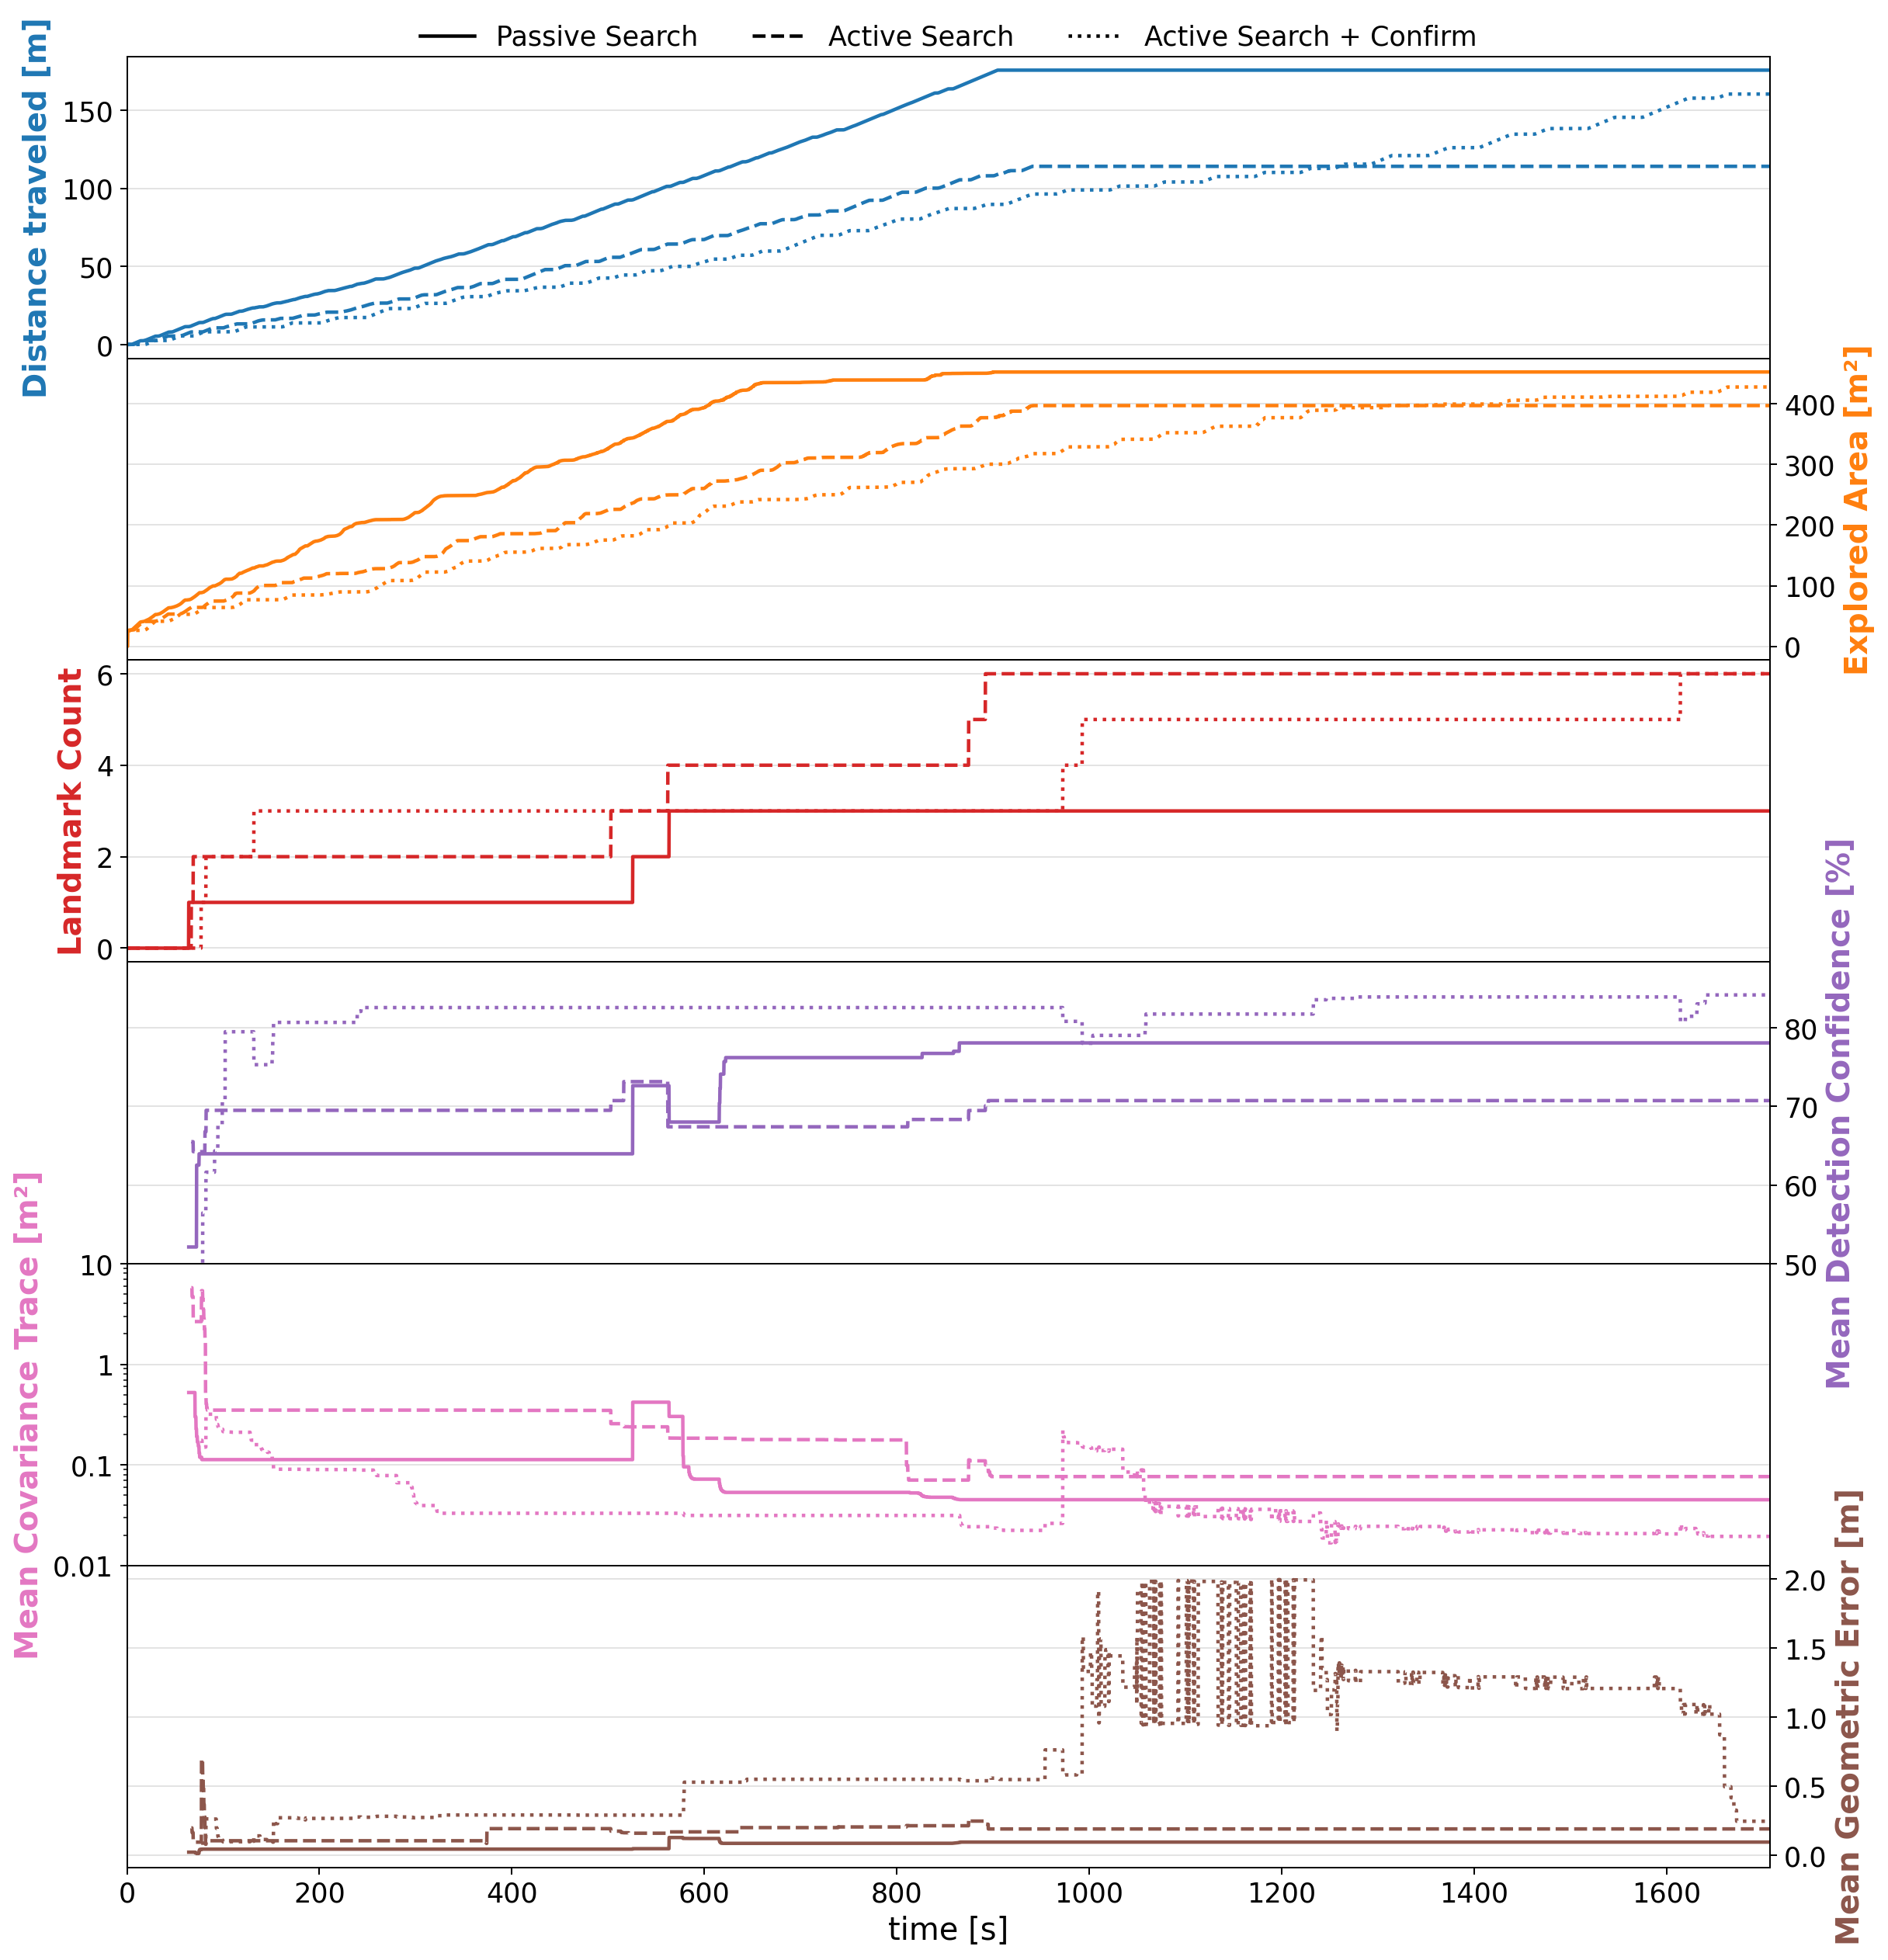
\includegraphics[width=0.95\textwidth]{assets/results_spot_chart.png}

    \caption{Comprehensive timeline of evaluation metrics recorded during the physical deployment of the Boston Dynamics Spot robot in the office environment. The stacked subplots track distance traveled, cumulative battery discharge, explored area, landmark count, mean detection confidence, and mean covariance trace (logarithmic scale). The evaluated strategies are Passive Search (solid line), Active Search (dashed line), and Active Search with Confirmation (dotted line).}

    \label{fig:res_spot_chart}

\end{figure} 

\cleardoublepage

% List of figures (optional) - useful over 3-5 figures
% \phantomsection
% \addcontentsline{toc}{chapter}{\lstfigurelabel}
% \listoffigures
% \cleardoublepage

% List of tables (optional) - useful over 3-5 tables
% \phantomsection
% \addcontentsline{toc}{chapter}{\lsttablelabel}
% \listoftables
% \cleardoublepage

% List of algorithms (optional) - useful over 3-5 algorithms
% \phantomsection
% \addcontentsline{toc}{chapter}{\lstalgorithmlabel}
% \listofalgorithms
% \cleardoublepage

% List of codes (optional) - useful over 3-5 code samples
% \phantomsection
% \addcontentsline{toc}{chapter}{\lstcodelabel}
% \lstlistoflistings
% \cleardoublepage

% List of symbols (optional)
%\printnomenclature

\end{document}% this document is based on Máté Cserép https://github.com/mcserep/elteikthesis work and Zoltán Istenes modifications, extensions (2023), specially created for the IFRoS students